\documentclass[]{UCD_CS_47360_Report}
\usepackage{graphicx}
\usepackage{hyperref}
\usepackage{amsmath}


%%%%%%%%%%%%%%%%%%%%%%
%%% Input project details

\def\studentname{Daniel Danev, Turlough Hannon, Adam Ryan, Danning Zhan} % Edit with your names
\def\projecttitle{Predicting Dublin Bus Journey Times} % Edit with your project title
\def\groupnum{10} % Edit with your group number

%\begin{article}
\begin{document}

\maketitle

%%%%%%%%%%%%%%%%%%%%%%
%%% Your Project Specification

\chapter*{Project Specification}


Bus companies produce schedules which contain generic travel times. For example, in the Dublin Bus Schedule, the estimated travel time from Dun Laoghaire to the Phoenix Park is 61 minutes (\href{http://dublinbus.ie/Your-Journey1/Timetables/All-Timetables/46a-1/}{http://dublinbus.ie/Your-Journey1/Timetables/All-Timetables/46a-1/}).

Of course, there are many variables which determine how long the actual journey will take. Traffic conditions which are affected by the time of day, the day of the week, the month of the year and the weather play an important role in determining how long the journey will take. 

These factors along with the dynamic nature of the events on the road network make it difficult to efficiently plan trips on public transport modes which interact with other traffic. 

This project involves analysing historic Dublin Bus data and weather data in order to create dynamic travel time estimates. 

Based on data analysis of historic Dublin Bus data, a system which when presented with any bus route, departure time, the day of the week, current weather condition, produces an accurate estimate of travel time for the complete route and sections of the route. 

Users should be able to interact with the system via a web-based interface which is optimised for mobile devices. When presented with any bus route, an origin stop and a destination stop, a time, a day of the week, current weather, the system should produce and display via the interface an accurate estimate of travel time for the selected journey

%%%%%%%%%%%%%%%%%%%%%%
%%% Your Abstract here

\begin{abstract}


Dublin Bus provides commuters with bus schedules and generic travel times through their website and mobile application. In reality travel times are not static and vary along identical routes depending on a variety of factors including the weather, time and day of the journey, and events which may occur all of which result in generic journey times being poorly suited in informing commuters. 

This paper charts the development of a Flask-based web application which incorporates Random Forest models trained using historical bus and weather data in order to create dynamic travel time predictions for Dublin Bus journeys. Through the usage of an Agile and Scrum framework to manage development, Microsoft Azure to host application data, Flask to serve as the application back-end, and Vue to provide responsive front-end features, we deploy a modular Dublin Bus travel time prediction application using a modern development framework. This application not only provides users with travel time predictions based on route information and location information but also it incorporates a number of additional features including a favourite trip system, a weather feed integration, a Twitter feed integration, multiple colour themes, and an innovative sustainability-focused points system. The paper discusses the implementation of these features, and outlines considerations for future implementation.

\section*{Acknowledgments}


We would like to express our thanks to all of the mentors that set us on our path for this project. We are grateful for the feedback and direction we received during each of the mentor meetings. We wish to express a thank you to all of our team mates and to the project supervisors for their insight into our ideas and for their guidance throughout the project.

\end{abstract}
%%%%%%%%%%%%%%%%%%%%%%
%%% Acknowledgments




%%%%%%%%%%%%%%%%%%%%%%
%%% Table of Content

\tableofcontents\pdfbookmark[0]{Table of Contents}{toc}\newpage
\newpage


%%%%%%%%%%%%%%%%%%%%%%
%%% Introduction

\chapter{Introduction}

Dublin Bus was founded in 1987 and maintains a bus network which operates in the Greater Dublin Area and extends to Wicklow and Kildare \cite{DublinBus-About}, maintaining over 136 routes in this region \cite{TFI-BusTravel}. Dublin Bus provides users with a Journey Planner \cite{DublinBus-JourneyPlanner} and Timetable \cite{DublinBus-Schedule} which provide estimated journey times; however, there is extensive literature showcasing that bus journey times are variable and impacted by a variety of factors including weather, passenger volumes, travel distance, and time of travel \cite{Diab:2013}. Not only is accurate travel time important for travellers in helping to minimise wait times and accurately plan journeys, but it is also important to service operators as provision of accurate travel times is correlated with consumers' willingness to pay and perception of the service \cite{Zheng:2010}. For many users the travel time service provided by Dublin Bus is inadequate; it is frequently cited by users as a key driver in their poor perception of Dublin Bus's offering in addition to other key drivers such as having an "outdated UX", showing "no signs of being updated", and being "slow and not user friendly." \cite{DublinBus-Reviews} \cite{DublinBus-Reviews-2} \cite{DublinBus-Reviews-3}. 

A variety of modelling methodologies have been attempted to address the variability of travel times in literature. Researchers have experimented with modelling methods including Random Forests based on Near Neighbours (RFNN) \cite{Yu:2018}, Convolutional LSTM Neural Networks \cite{Petersen_2019}, Support Vector Machines (SVM) \cite{SVM}, and classical Random Forest (RF) \cite{RF} in attempts to accurately predict travel times and delay times for bus journeys throughout the world. Similarly, multiple applications exist for the purpose of improving other elements (e.g. UX) which are criticised in the Dublin Bus application including the TFI Real Time Planner \cite{TFI-App}, Google Maps \cite{GoogleMaps-App}, and Moovit \cite{Moovit-App} however these existing solutions have similarly received a range of responses with criticisms largely pertaining to UX elements, and journey time accuracy \cite{TFI-Review} \cite{GoogleMaps-Review} \cite{Moovit-Review}.

By developing a web application which leverages features and design choices of applications which are associated with positive perception based on user reviews, supporting these features through the development of machine learning models trained on 2018 bus and weather data to enable an increased accuracy in travel time predictions, and incorporating new innovative features to distinguish the application, the authors aim to develop an application which addresses both the inaccuracy of the travel times provided by Dublin Bus and the UX criticisms of existing solutions.

Using an Agile framework and the Scrum methodology \cite{Scrum-Guide}, a web application was developed by the four authors wherein roles were divided into front-end developer, back-end developer, data analyst, and a full-stack developer to align with key developer roles in industry \cite{SO-Survey} with the division of roles driven both by preference and prior experience in the role.

In the following sections the authors will chart an overview of the final application which was developed and the key features which were implemented by the authors, our approach to developing the application and the techniques administered in order to collaborate as a team, the tech stack and architecture of our application detailing design decisions which were made during development, our methods of evaluating and testing our application to assess its effectiveness against the project aims, and individually written components in which we will discuss our key contributions, understanding of the literature, and our evaluation of the project.

\chapter{\label{chapter2}Description of Final Product}
\section{Overview}
The final product is a web application usable on mobile and desktop devices. By choosing either a bus route with an origin and destination stop, or their planned departure location and destination location, users are presented with
\begin{itemize}
    \item A dynamic journey time based on the weather and route of their journey based upon a Random Forest model corresponding with their route to address the variability of bus journeys.
    \item A view of the journey on an embedded map to easily understand the path of the journey.
    \item Information on the necessary travel steps for their chosen trip for ease of travel.
    \item The current weather in Dublin and the seven day weather forecast for Dublin for a unified view of the journey.
    \item Dublin Bus's Twitter to identify real-time updates which may affect travel times.
\end{itemize} 
In addition to features developed to address the problem of accurate travel times, the application also contains quality of life enhancements and user retention features including
\begin{itemize}
    \item An opportunity to create an account enabling the ability to
    \begin{itemize}
        \item Take a presented trip for the purpose of acquiring points for that journey to aid in retention. 
        \item Saving routes for future access for ease of use.
        \item Remove their account if the application is no longer needed to provide trust.
    \end{itemize}
    \item A light and dark theme.
    \item An export to calendar function.
    \item Warnings when a model is unavailable or stops are not found.
\end{itemize} 
These features will be highlighted in more detail in the following sections.

\section{Key Features}

\subsection{Search Features}

The first search method detailed in \ref{fig:SearchByRoute} is the ability for a user to search by a specific route. A user selects the bus stop they want to travel from and the destination stop. The map will display the path the bus will take on the route. The user will receive information on the expected arrival time at each bus stop in their journey.

\begin{figure}[!htb]
    \centering
    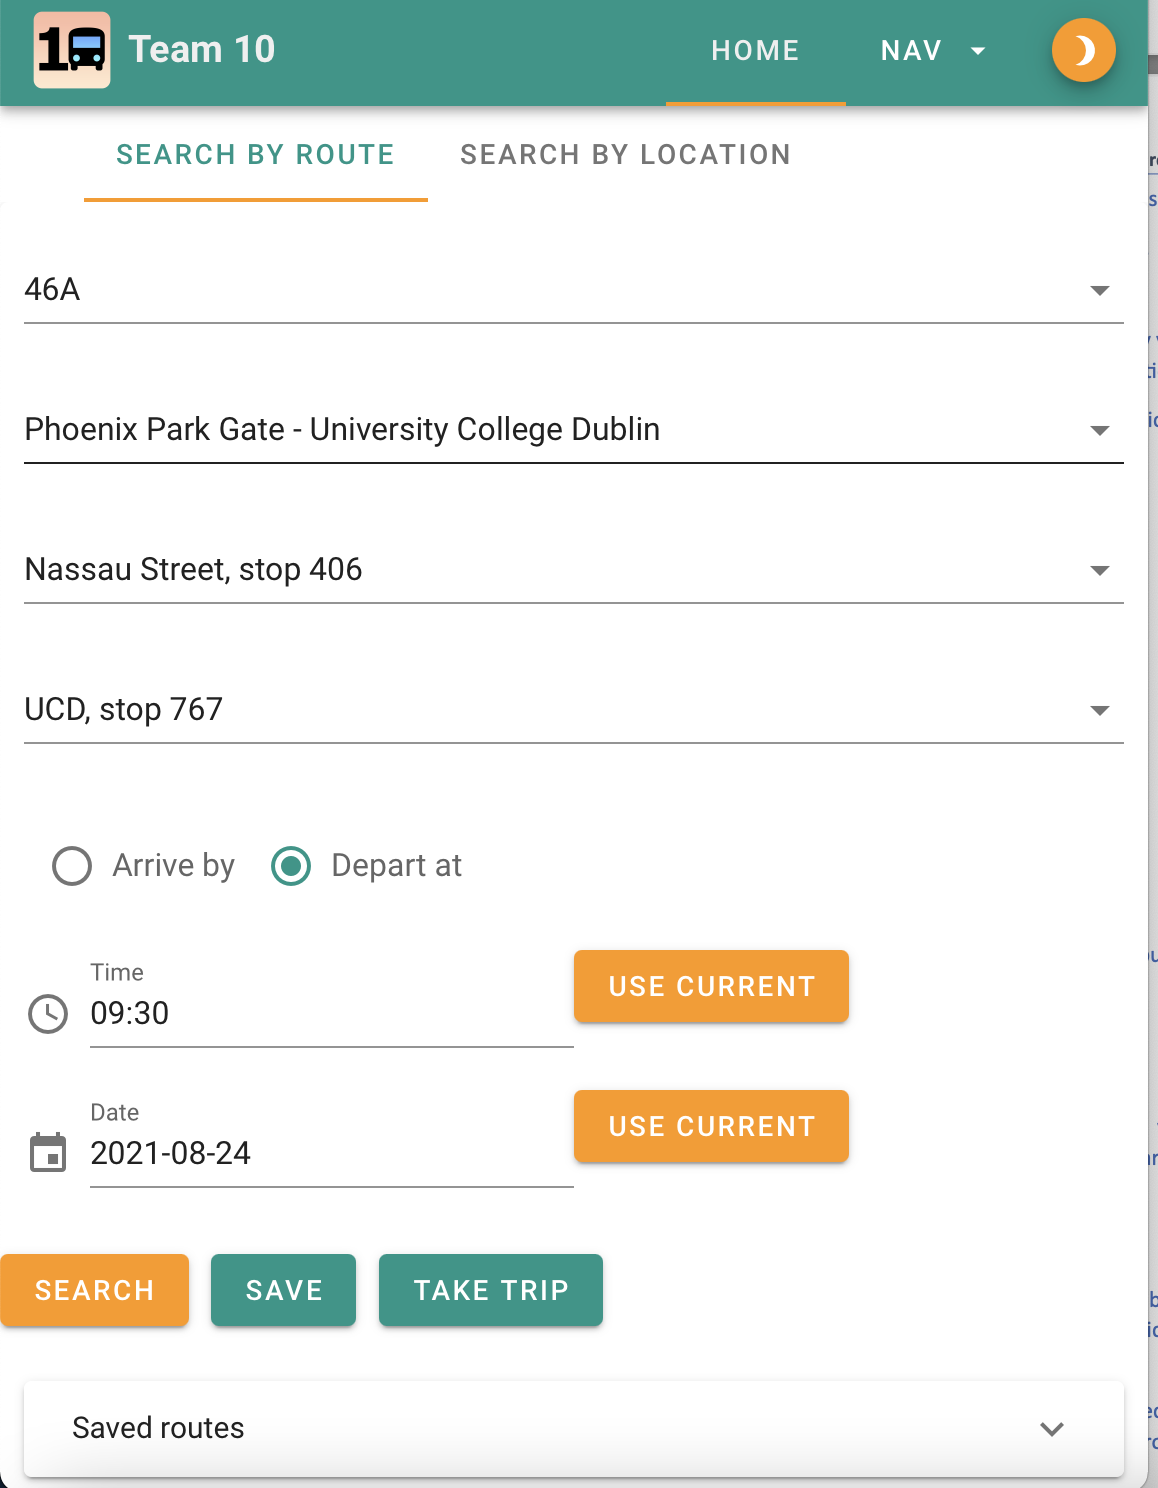
\includegraphics[width=0.3\textwidth]{figures/2_2_Search_By_Route_1.png}
    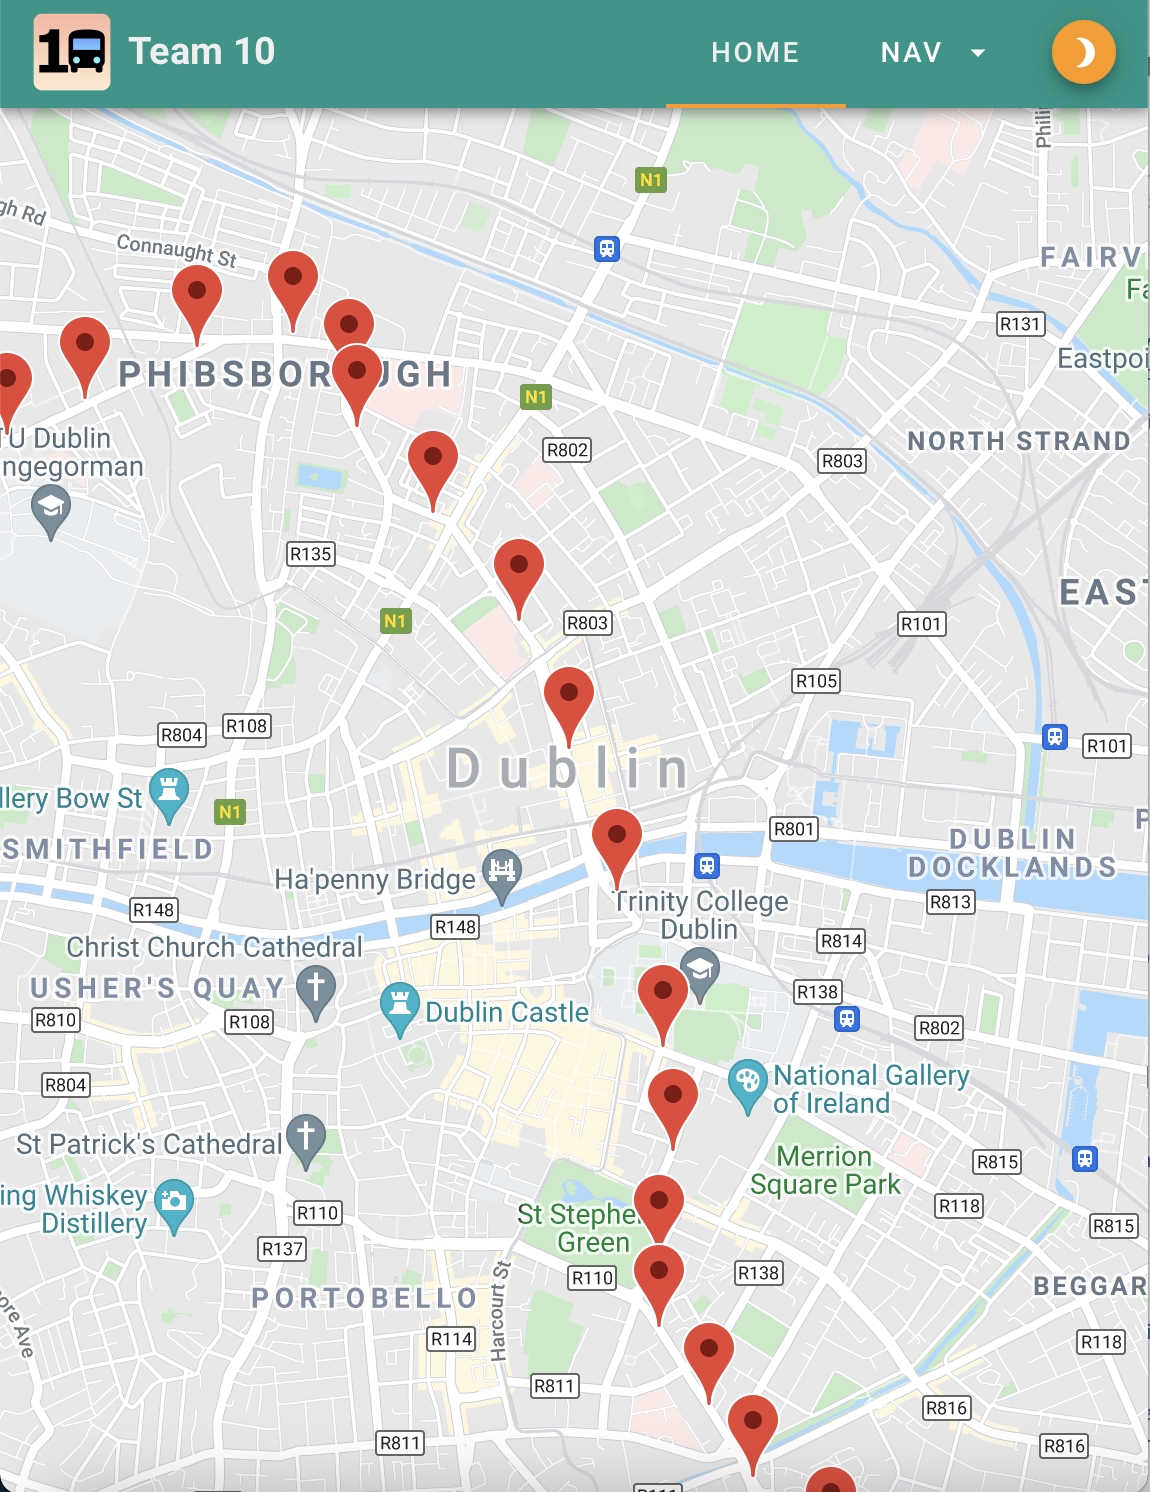
\includegraphics[width=0.3\textwidth]{figures/2_2_Map_View.png}
    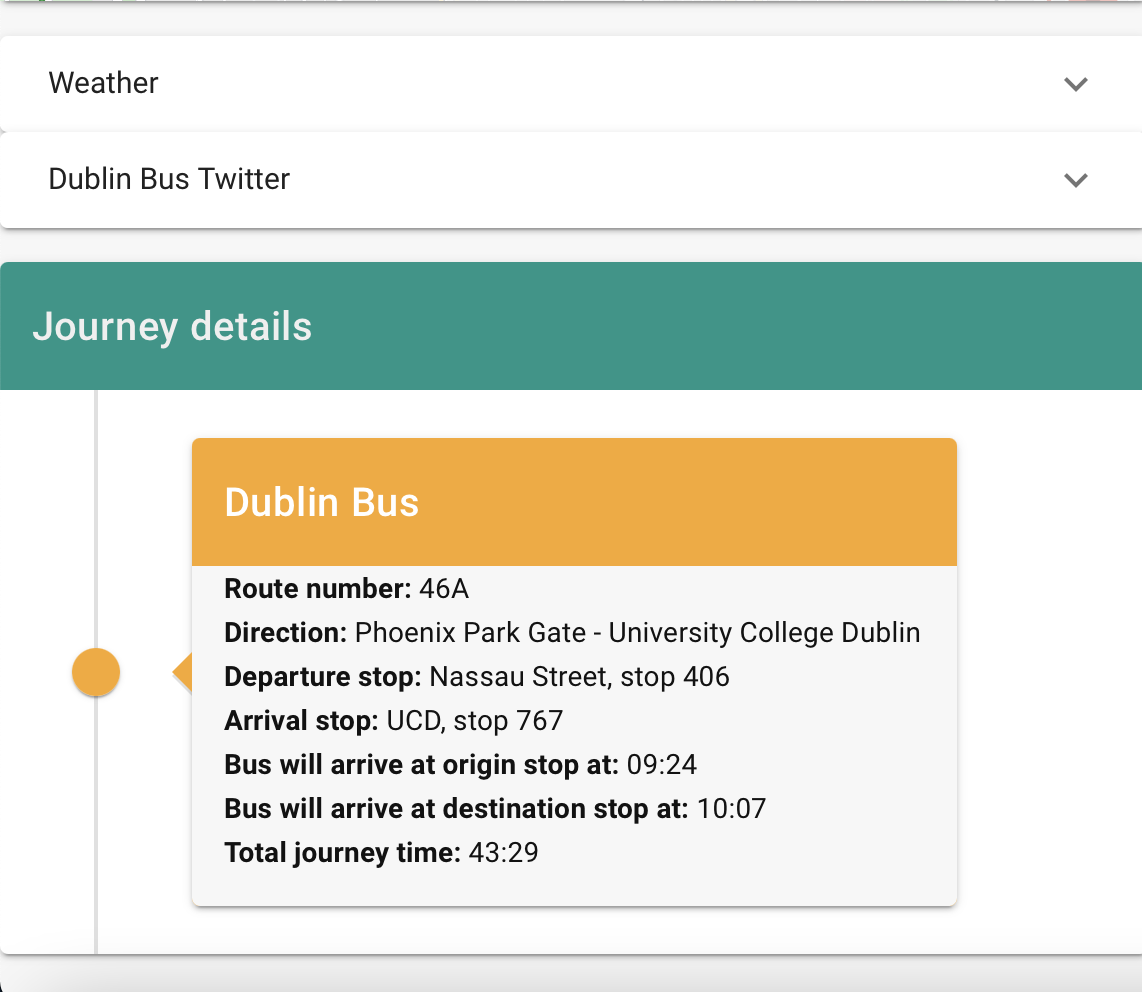
\includegraphics[width=0.3\textwidth]{figures/2_2_Search_By_Route_2.png}
    \caption{Search by Route}
    \label{fig:SearchByRoute}
\end{figure}

The second search method detailed in \ref{fig:SearchByLocation} is the ability for a user to using their starting location and final location. The user can insert an origin and destination, and the map will display this route on the map.
\begin{figure}[!htb]
    \centering
    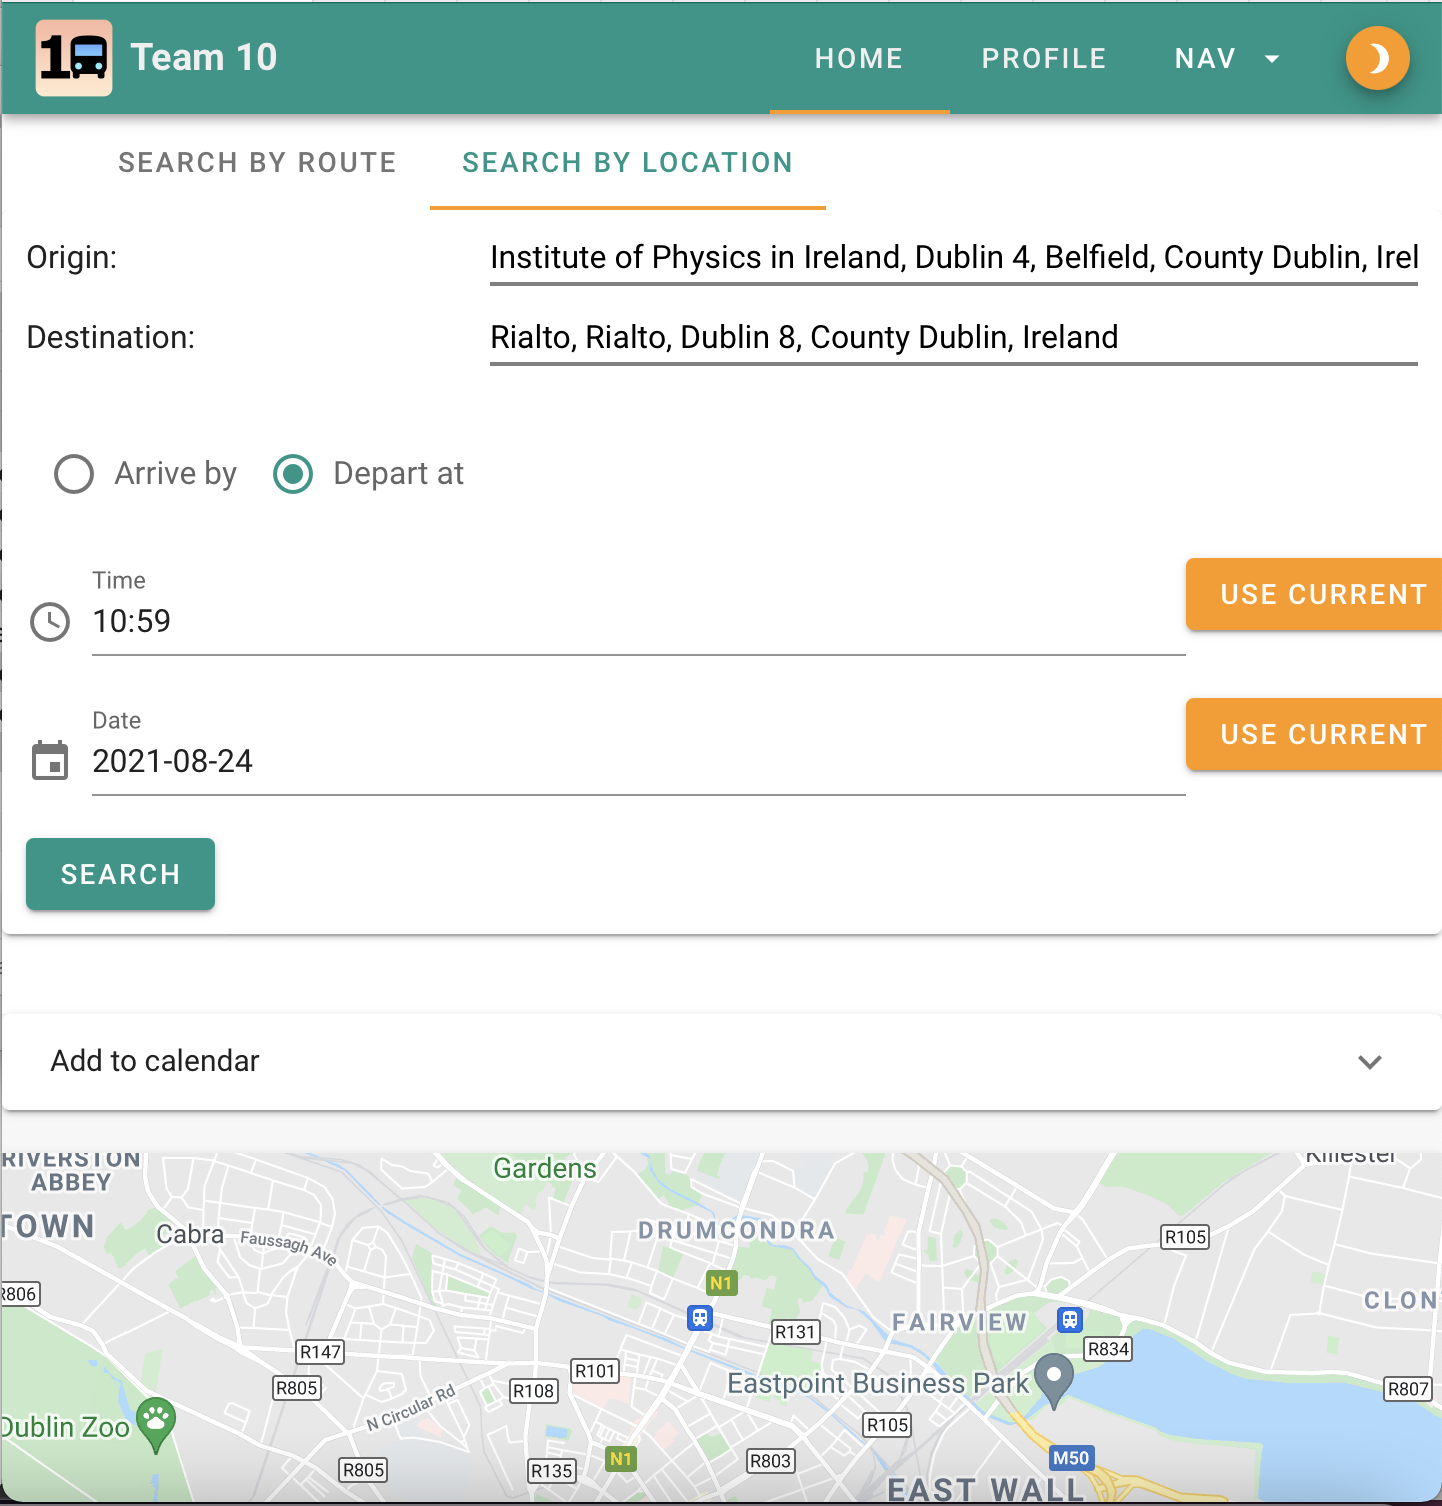
\includegraphics[width=0.3\textwidth]{figures/2_2_Search_By_Location_1.png}
    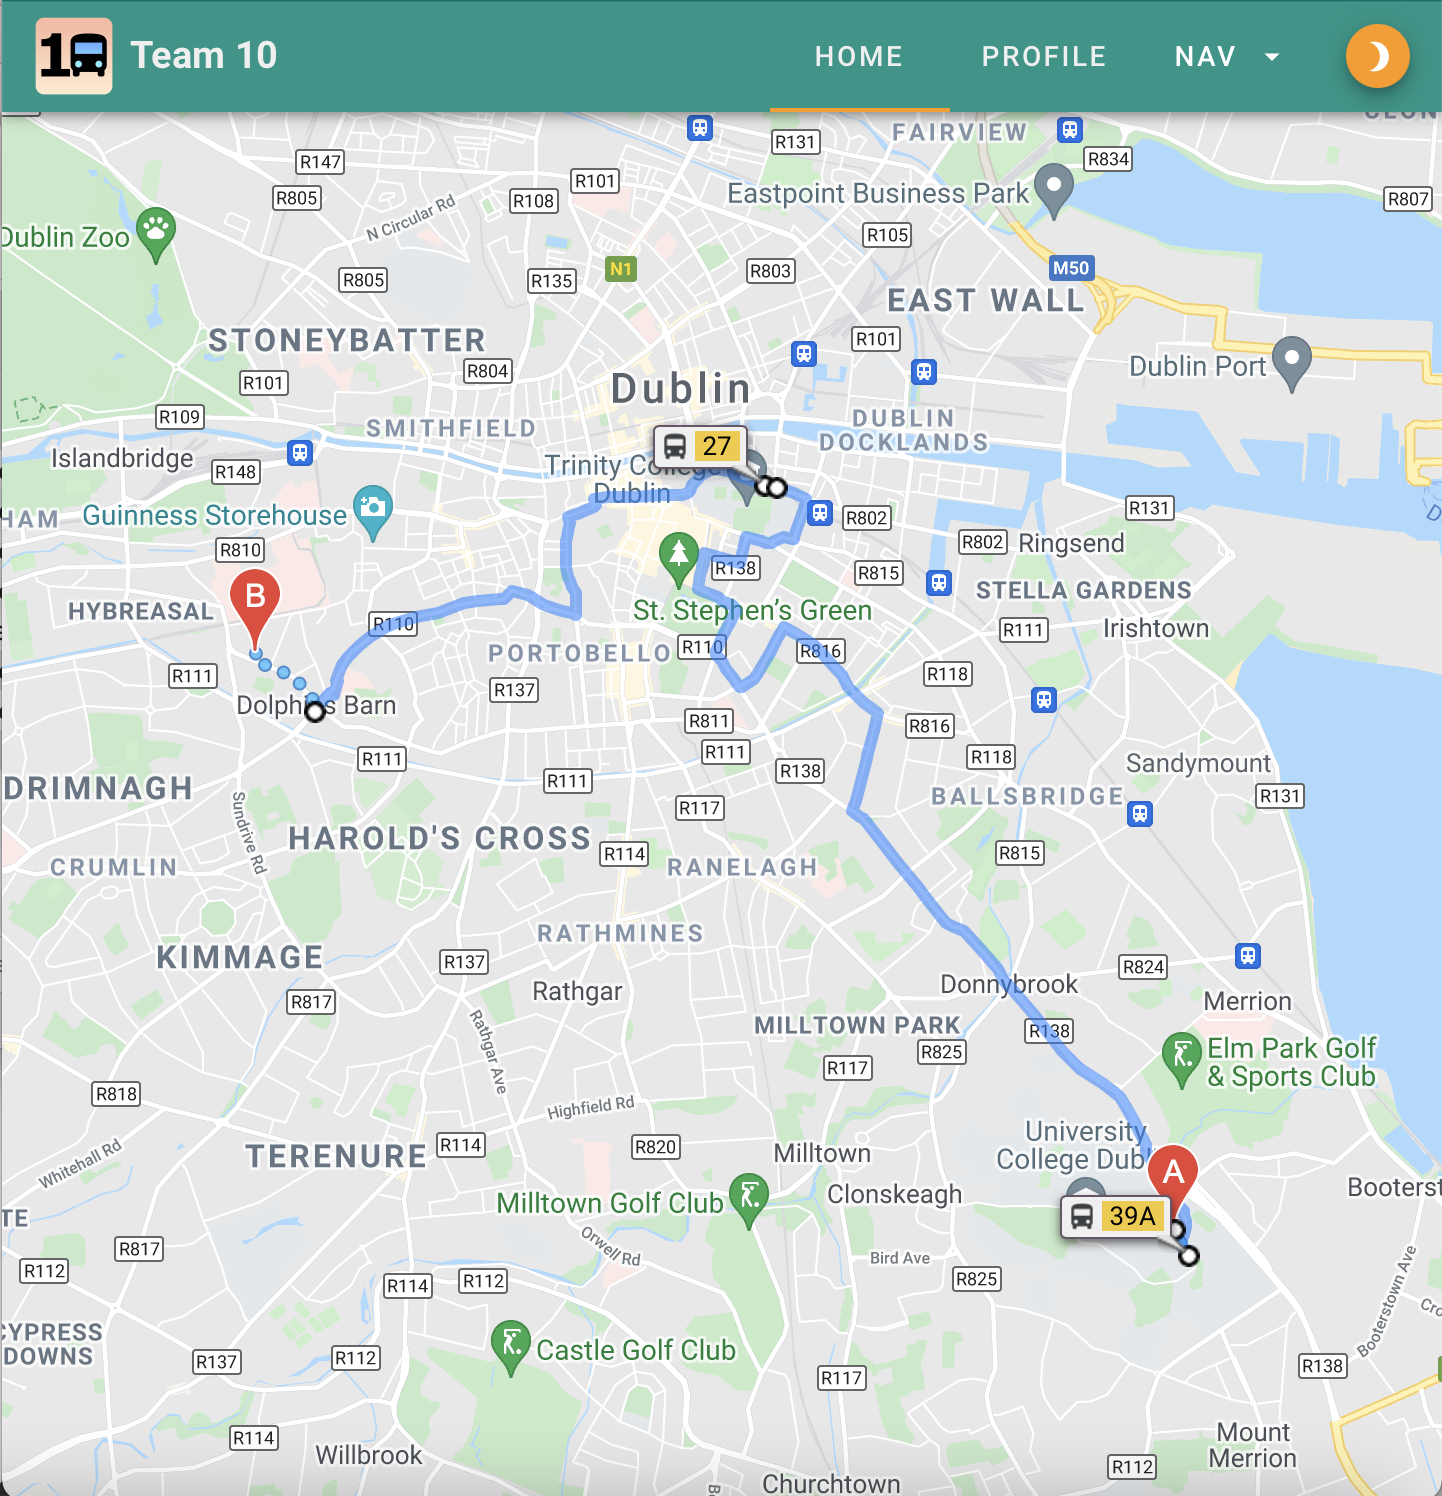
\includegraphics[width=0.3\textwidth]{figures/2_2_Map_View_2.png}
    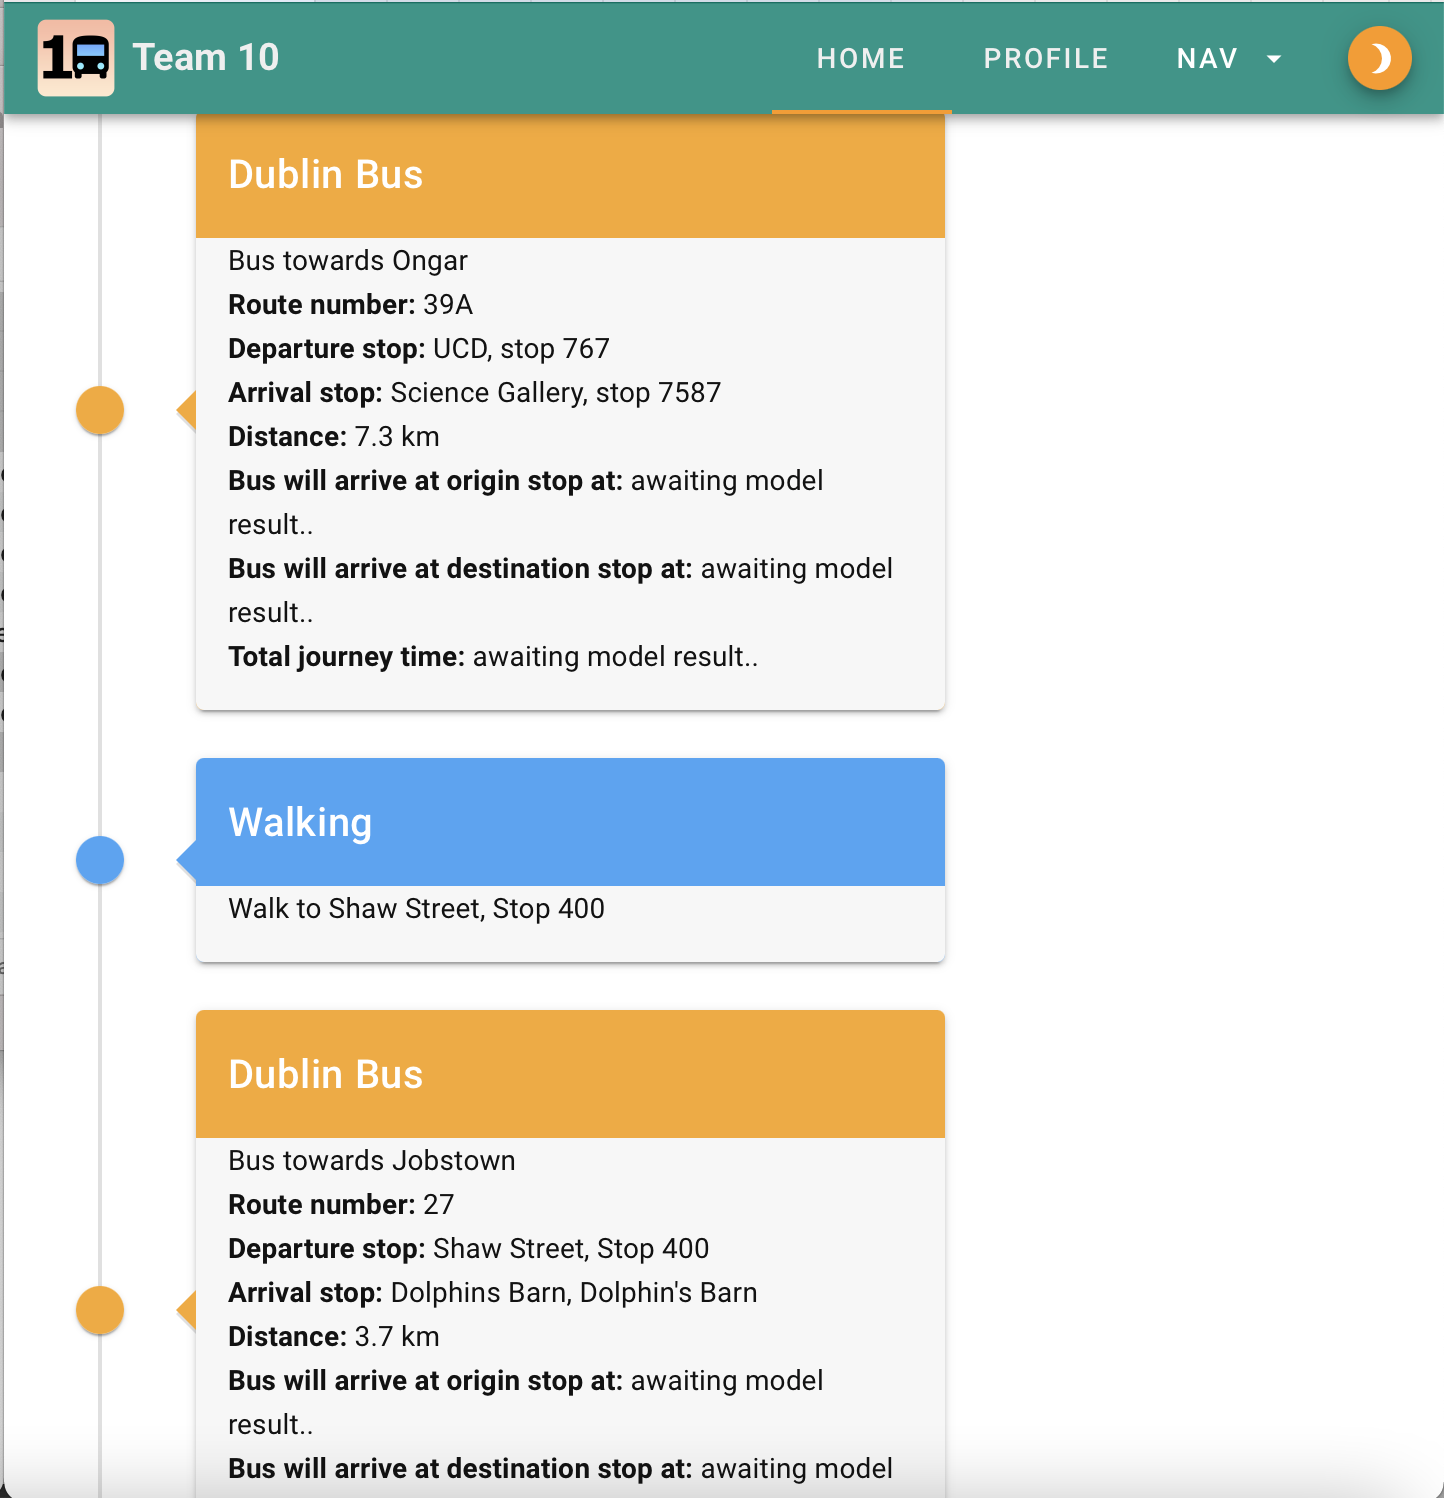
\includegraphics[width=0.3\textwidth]{figures/2_2_Search_By_Location_2.png}
    \caption{Search by Location}
    \label{fig:SearchByLocation}
\end{figure}

In both instances, the user input is passed from the front-end into the Random Forest models which were trained and saved in the application. The model predicts the bus's anticipated delay time at each of the stops so that the application calculate the overall journey time. The journey time is then calculated and displayed to the user, in addition to the expected arrival time of the bus at each stop. As the model may take a few seconds to be called, the user is notified via an 'Awaiting Model Results' notice. Through this feature, we aim to improve upon the Dublin Bus static schedule times and directly tackle the challenge of providing dynamic journey times to users.


\subsection{Profile Features}
In order to provide users with a personalised experience tailored to their usage, the application includes a registration system where users can sign-up and subsequently sign-in to the application in order to enable additional functionality in the form of the favourite route functionality and the points system functionality.
\begin{figure}[!htb]
    \centering
    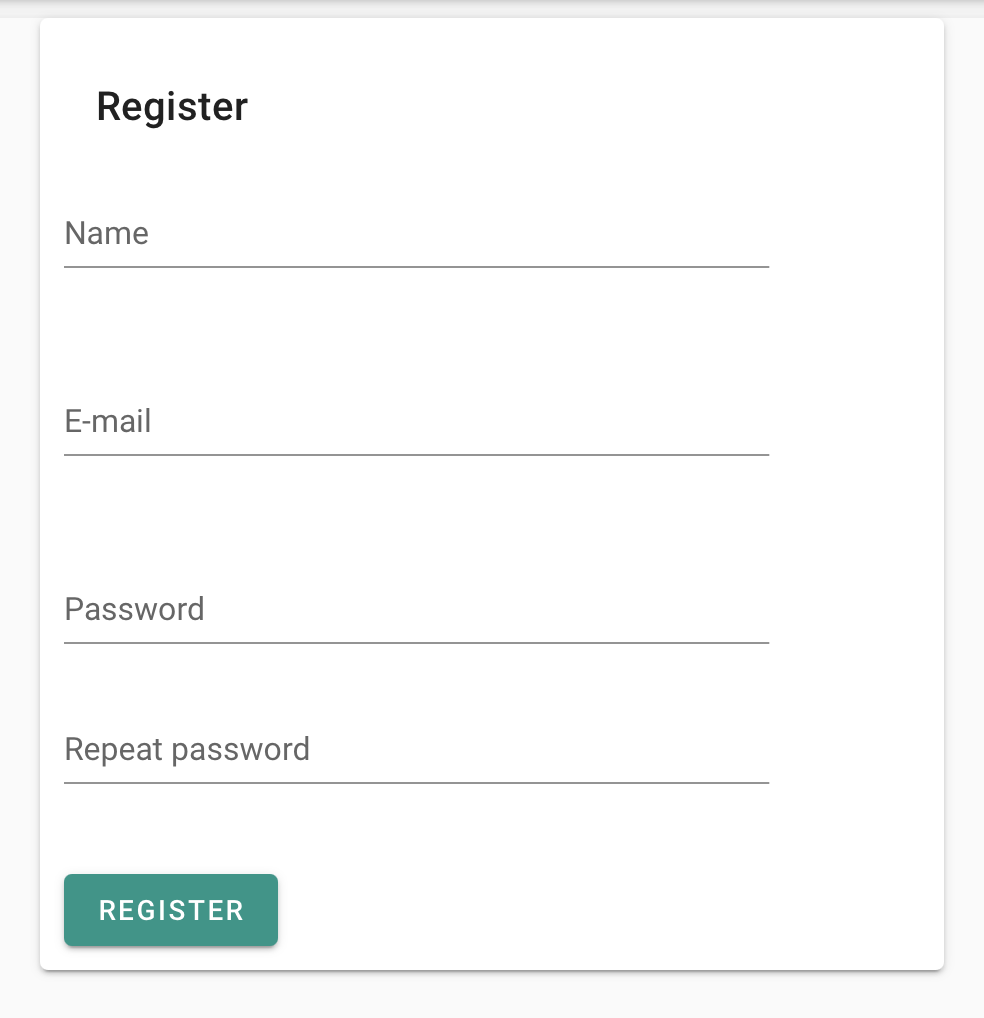
\includegraphics[width=0.4\textwidth]{figures/2_4_Register.png}
    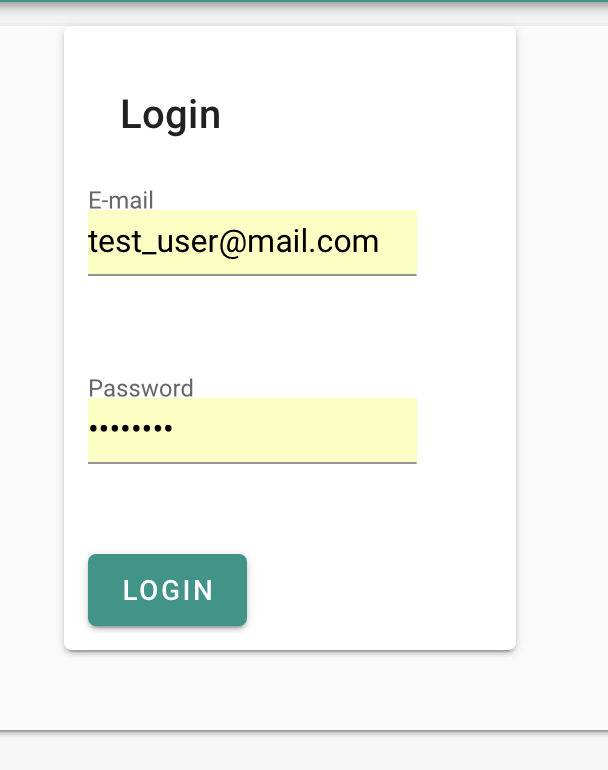
\includegraphics[width=0.4\textwidth]{figures/2_4_Login.png}
    \caption{Registration and Login Pages}
    \label{fig:Registration}
\end{figure}
As users may frequent certain routes in accordance with daily or weekly routines, and as it is a feature in well-rated applications such as Moovit, the team elected to implement a feature enabling logged-in users to save certain routes to their profile. These routes appear in a widget for the user to enable their favourite route, departure stop, and destination stop to be automatically inputted into the route form.
\begin{figure}[!htb]
    \centering
    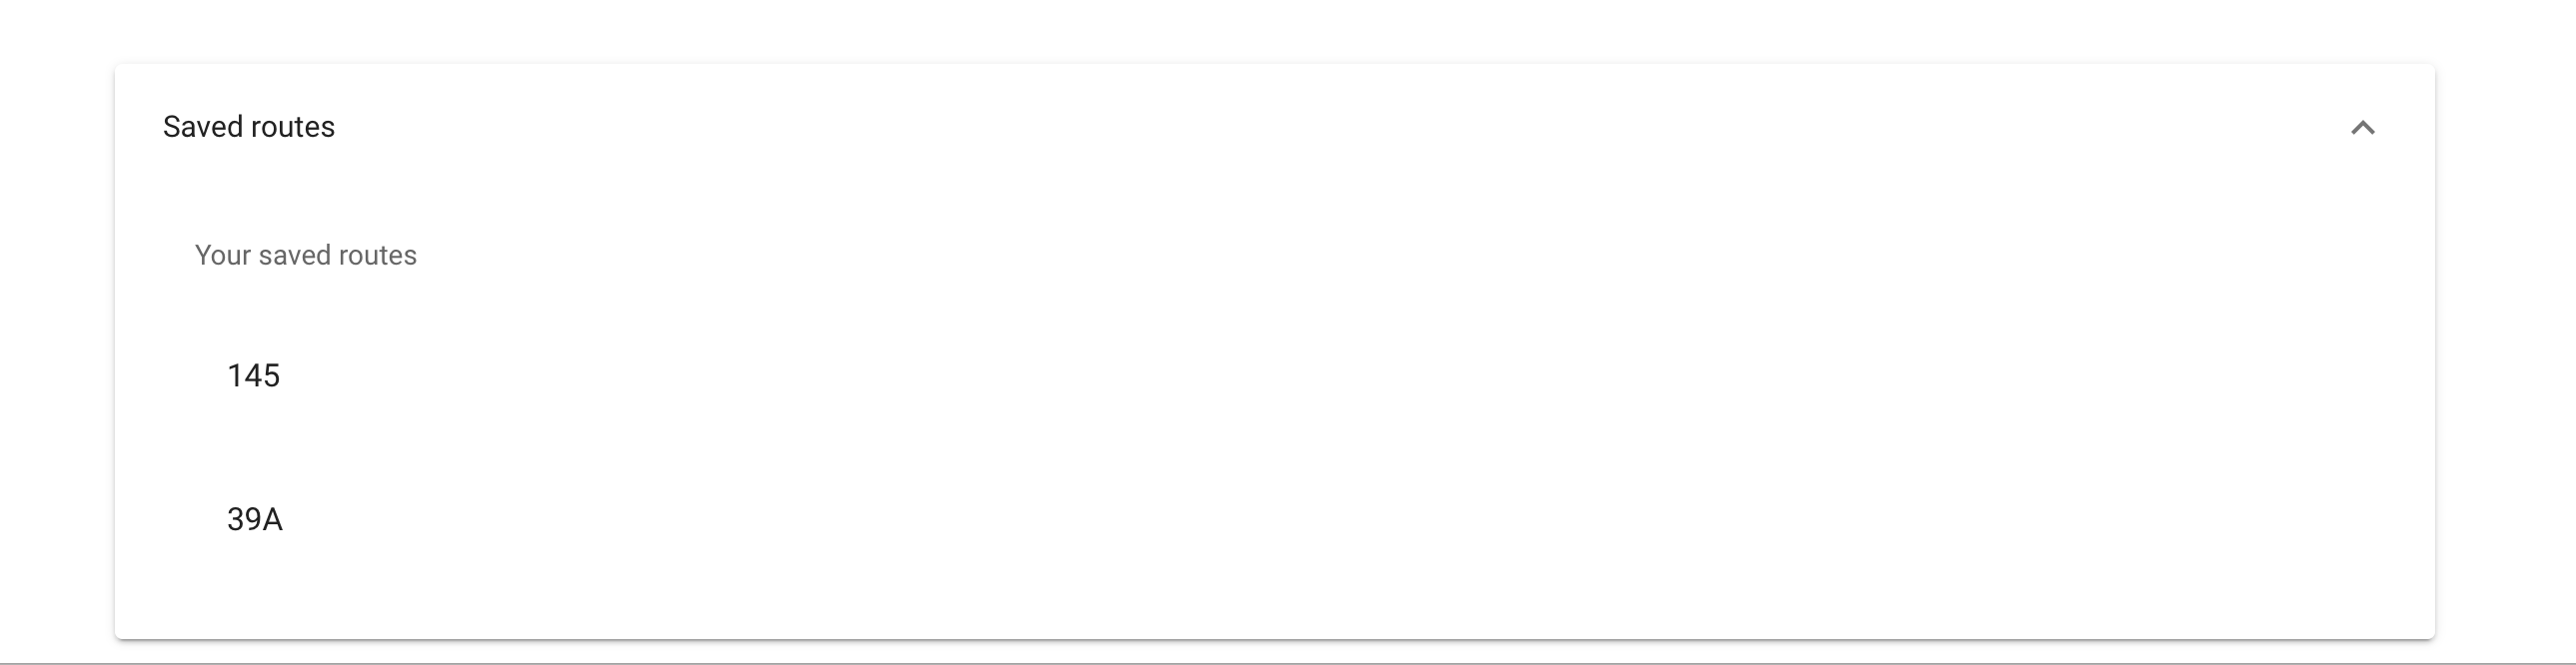
\includegraphics[width=0.5\textwidth]{figures/2_4_Saved_Routes.png}
    \caption{Favourite Routes}
    \label{fig:Registration}
\end{figure}

Gamification is an increasingly popular method in computer-human interaction to increase user retention and engagement with an application \cite{Gamification-Retention}. With sustainable environmental practices a topic of global concern and public transport a key method in reducing personal transport burdens \cite{IPCC}, a points system was integrated into the app which is rooted in the volume of carbon dioxide emissions that each person will emit for each trip, triggered once a user selects the button to take the trip.

By comparing bus emissions to private car emissions, we equated the difference between these methods to the $CO_2$ that an average tree would intake from the atmosphere and converting this to a points total. Explicitly this was calculated by assuming \cite{BBC-Car} \cite{Tree}:
\begin{itemize}
    \item A tree consumes $3$g/h of $CO_2$.
    \item A car emits $200$g/km of $CO_2$.
    \item A bus emits $100$g/km of $CO_2$ per passenger.
\end{itemize}
Therefore
\begin{itemize}
    \item $100$g/km in reduction per passenger $ \implies $  $33$hr reduction per tree per km travelled.
\end{itemize}
Using this logic, the developers decided to implement 33 points per kilometre (0.033pts/m) travelled to loosely correlate a user's points per journey to environmental impact. While it is understood that this operates under highly generalised assumptions, the key aspect of this feature is in the retention benefits and providing a motive for the user to engage in sustainable transportation methods, and the points calculation can be flexibly tuned and is integrated into the user's profile as in \ref{fig:PointsPerProfile}.

\begin{figure}[!htb]
    \centering
    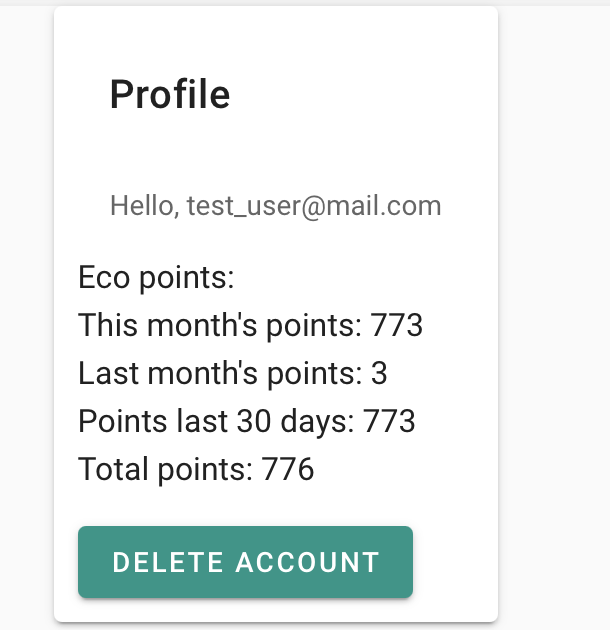
\includegraphics[width=0.3\textwidth]{figures/2_3_PointsPerProfile.png}
    \caption{Points Per Profile View}
    \label{fig:PointsPerProfile}
\end{figure}

While other applications feature points systems, the authors have been unable to identify an Irish bus journey application which integrates a points system based on environmental impact making this a uniquely innovative aspect of this application. In the event the user is not logged in and attempts to enable either feature, these are logged in our database as being saved against a guest profile with a user ID of '-1' to allow reporting on these events.

\subsection{Share Features}

The application includes the ability to share a trip with other users. The input parameters in the application are embedded into the URL upon search so that it may be shared with others. The application also features a method to add a trip to the user's calendar for integration into the user's other plans during a day or to share this calendar item with others. Through these features which extend beyond the brief, the application allows users to plan journeys together and adds a quality of life improvement which is present in some of the more highly rated travel applications such as Moovit \cite{Moovit-Review} and Google Maps \cite{GoogleMaps-Review}.

\subsection{Travel Context Features}
As weather is a key aspect of our Random Forest model due to the impact of rain on travel times, the application contains an hourly weather forecast over the next 48 hours, and a broader 7 day forecast in order for the user to prepare appropriately for their journey. Clear labelling and visualisations are provided to convey this to the user as detailed in \ref{fig:WeatherWidget}.
\begin{figure}[!htb]
    \centering
    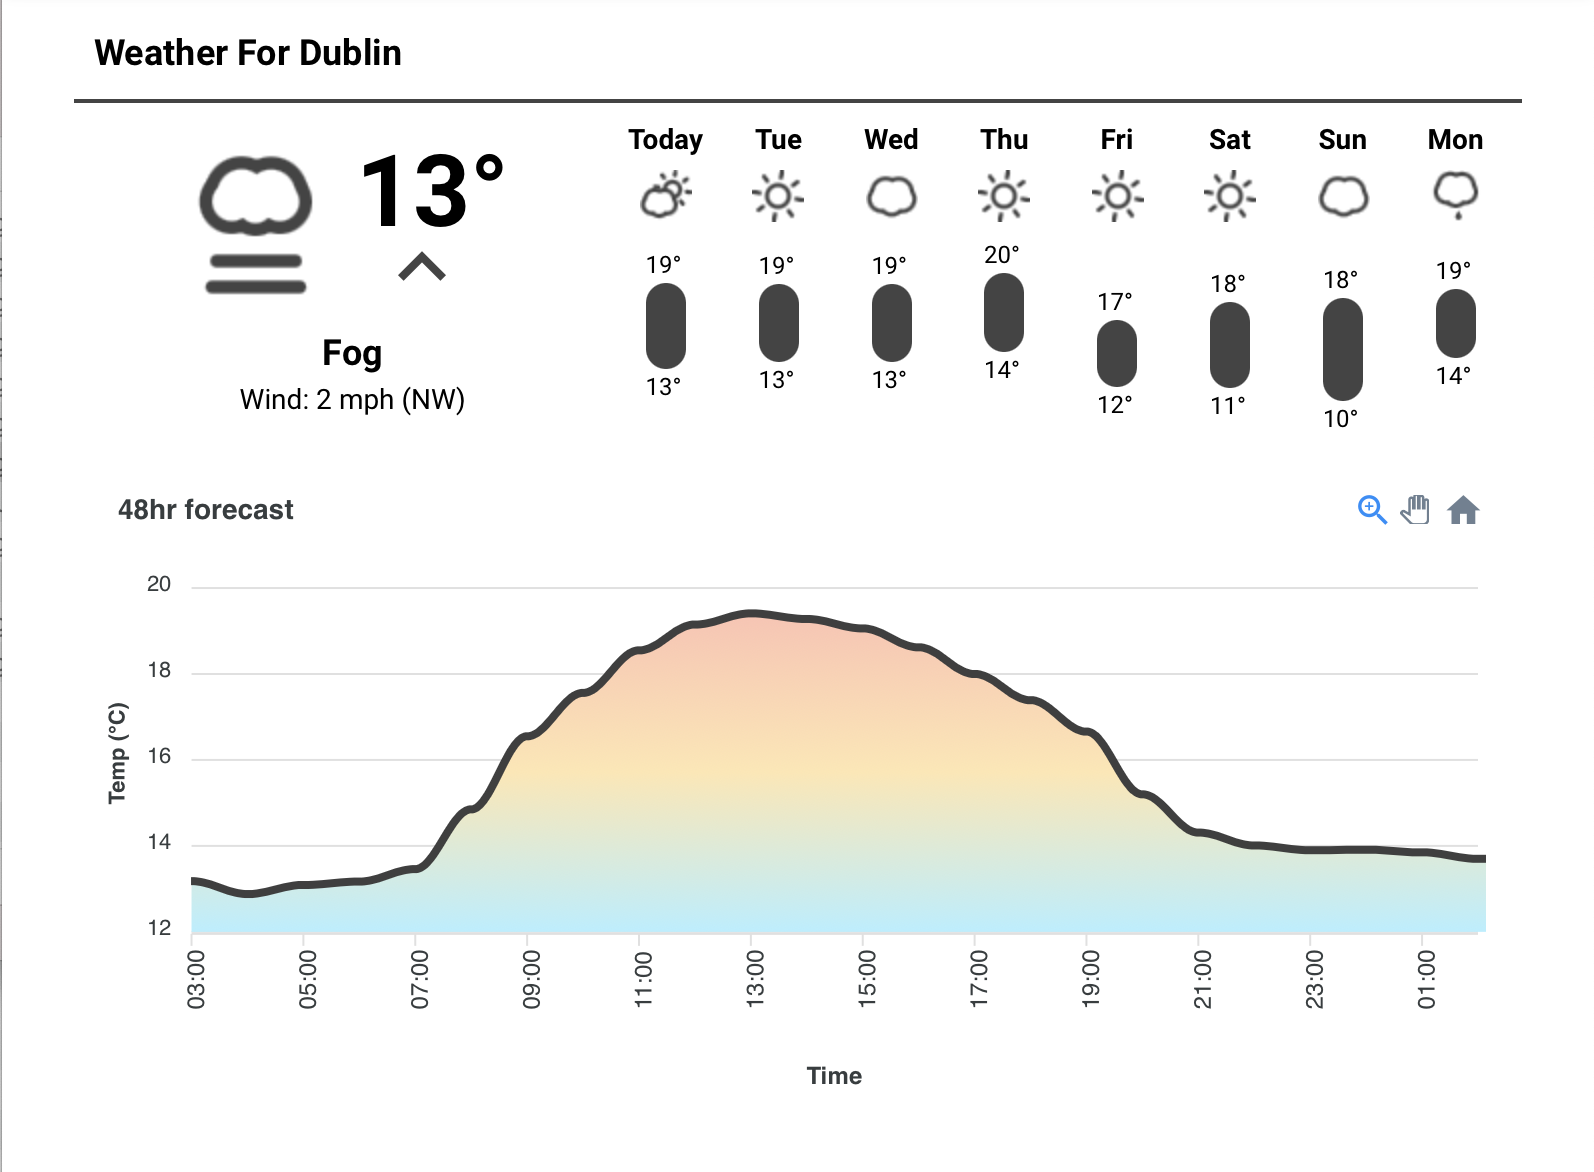
\includegraphics[width=0.3\textwidth]{figures/2_5_WeatherWidget.png}
    \caption{Weather Integration}
    \label{fig:WeatherWidget}
\end{figure}

As there are some events which cannot be foreseen by our implemented model, the team have identified that the most up-to-date source for rapid Dublin Bus news is their Twitter feed. In order for the user to immediately notice if there are any sudden changes that need to be made with regards to their plans, the developers have integrated Dublin Bus's bus feed into the application.
\begin{figure}[!htb]
    \centering
    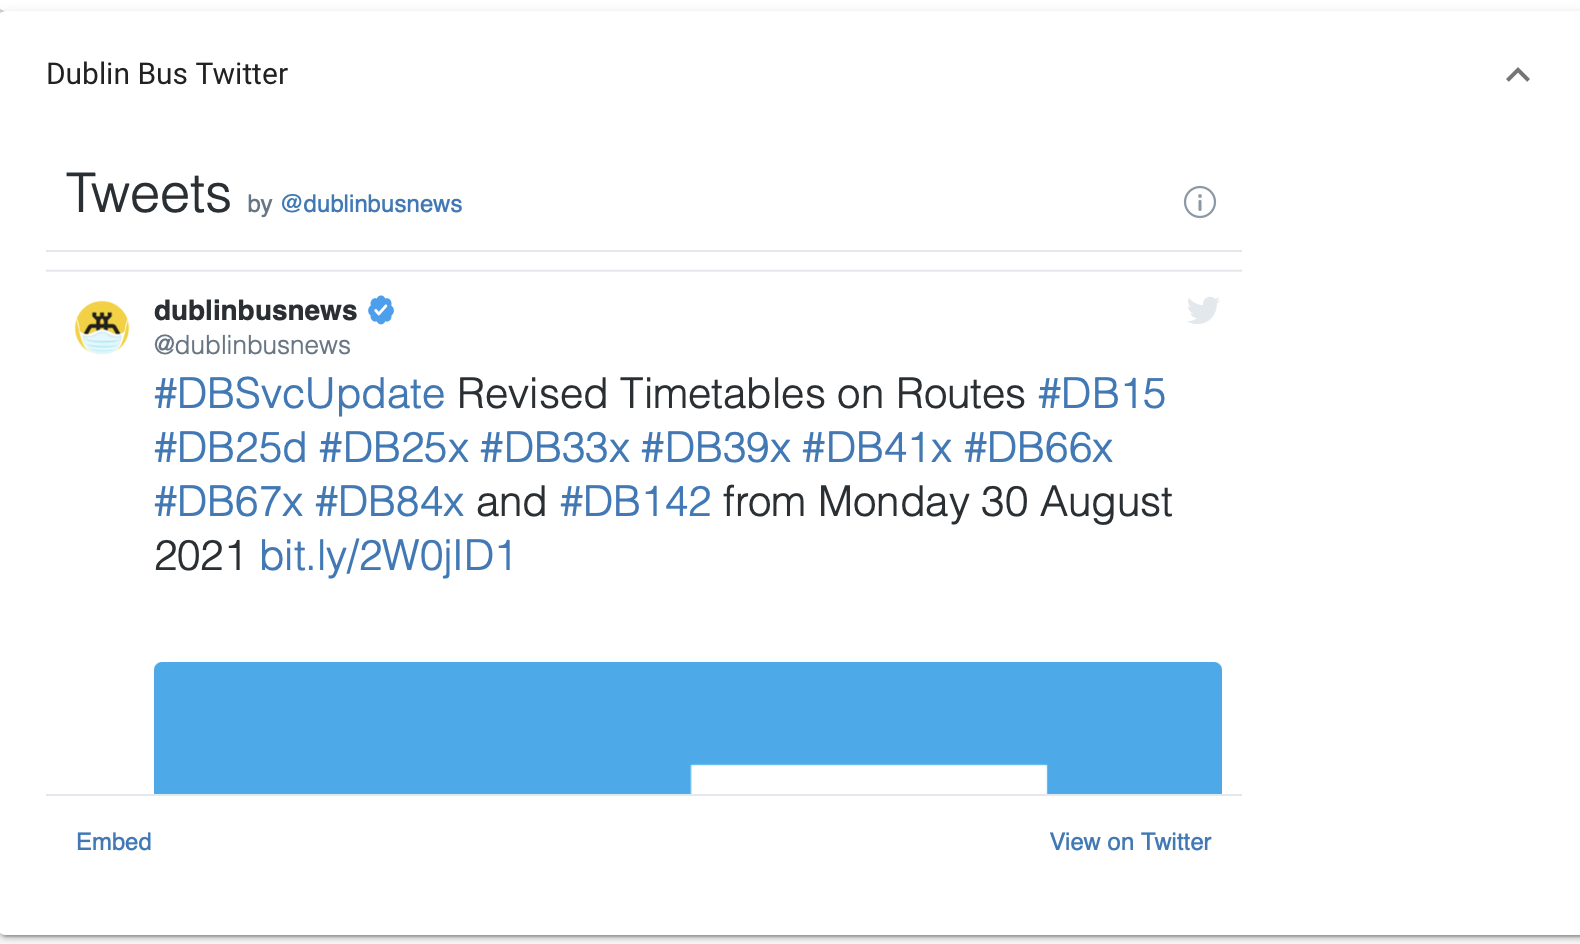
\includegraphics[width=0.3\textwidth]{figures/2_5_Tweets.png}
    \caption{Twitter Integration}
    \label{fig:Tweet}
\end{figure}

\subsection{User Interface}

To make the application more modern and user friendly, a dark and light mode has been implemented to assist in the alleviation of eye strain at different times of the day. 
\begin{figure}[!htb]
    \centering
    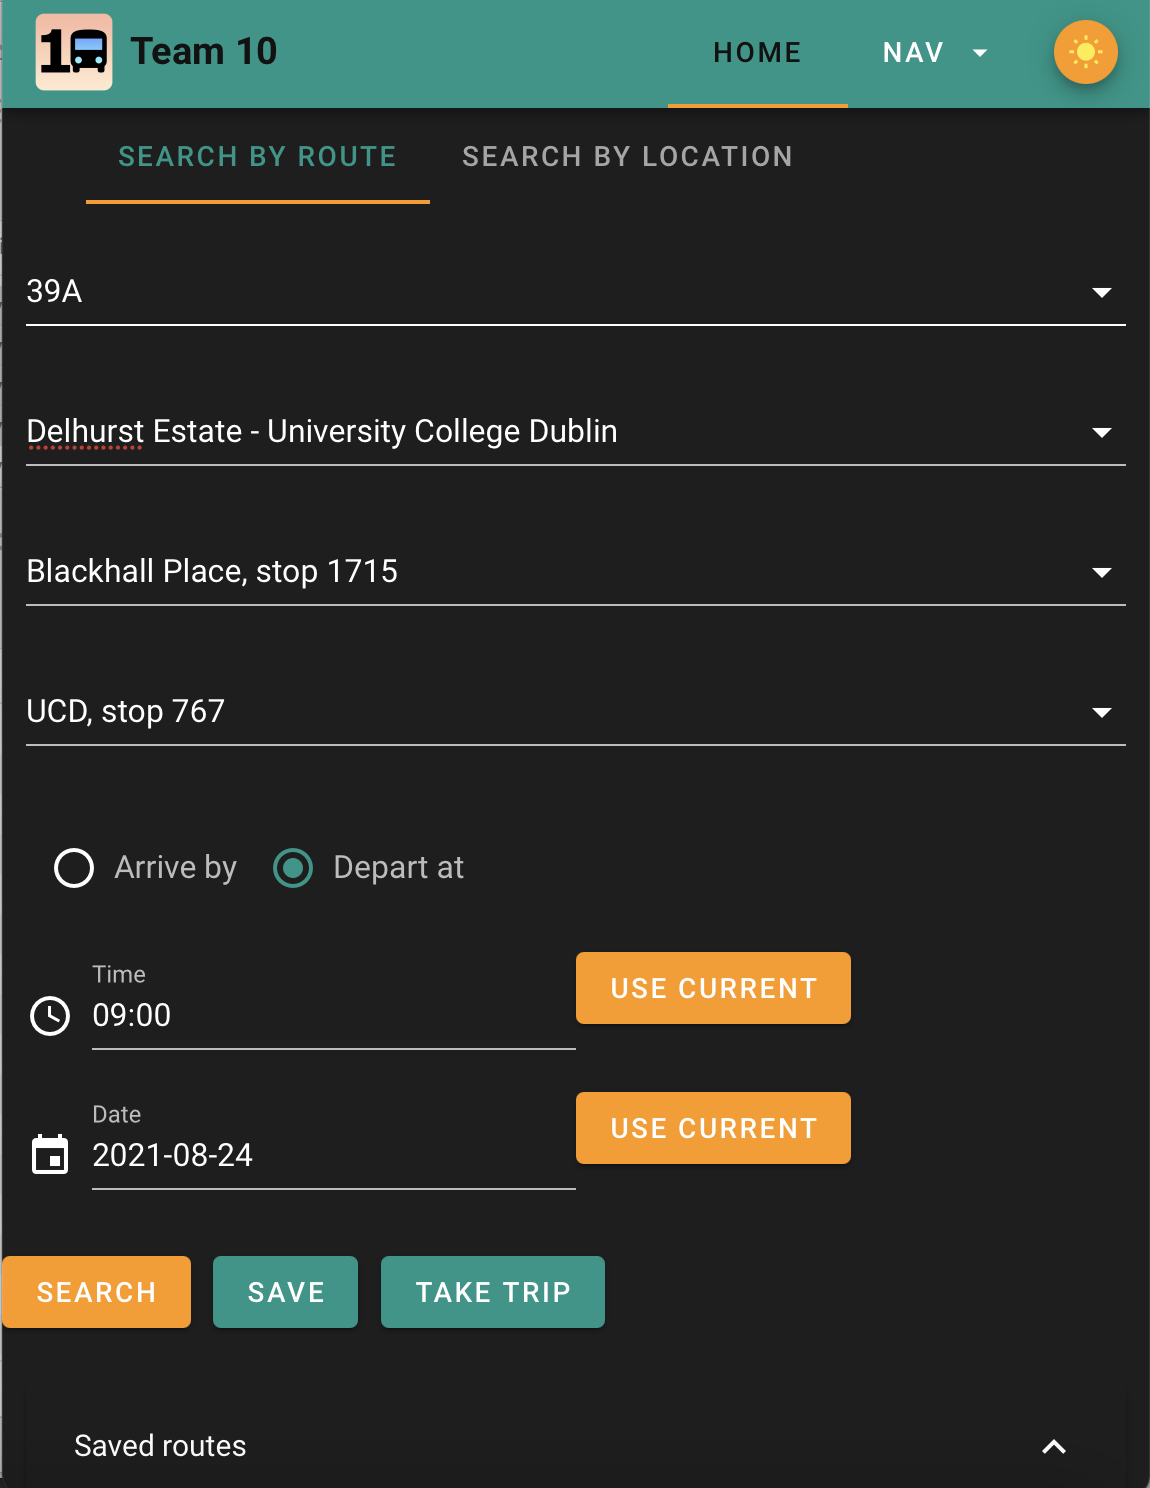
\includegraphics[width=0.4\textwidth]{figures/2_7_DarkMode.png}
    \caption{Dark Mode Theme}
    \label{fig:DarkModeTheme}
\end{figure}

The application has been built following responsive design principles and will adjust the application display based on the user's device.

\chapter{\label{chapter3}Development Approach}
Having examined the final web application, and identified some of the key application features which were implemented to address the task outlined in the project specification, this section will chart how the application arrived to its final state, charting the team's development and organisation approaches over the course of the project. 

Following standard industry practices the Scrum methodology \cite{Scrum-Guide} was used in the creation of the web application over a twelve week period. Each sprint was organised around the five presentations which were required as part of COMP47360 with the presentations dictating deadlines for key tasks to be complete for the purpose of the presentation.

The sprints employed broadly entailed:
\begin{enumerate}
    \item Setup, Requirements, and Exploration.
    \item Data Modelling
    \item Data Analytics
    \item Advanced Features
    \item Bug Fixing and Final Features
\end{enumerate}

Atlassian's software suite was used as the key project management tool to organise the team's development on the basis that its suite is used by 83\% of the Fortune 500 making it an industry-leader in project management software \cite{AtlassianUsage}. For our project, we incorporated Jira to track Epics and Tasks which required completion \cite{Epics}, and Confluence to document design decisions, meetings, and development information, with our Confluence structure outlined in \ref{fig:ConfluenceOverview}. 

\begin{figure}[!htb]
    \centering
    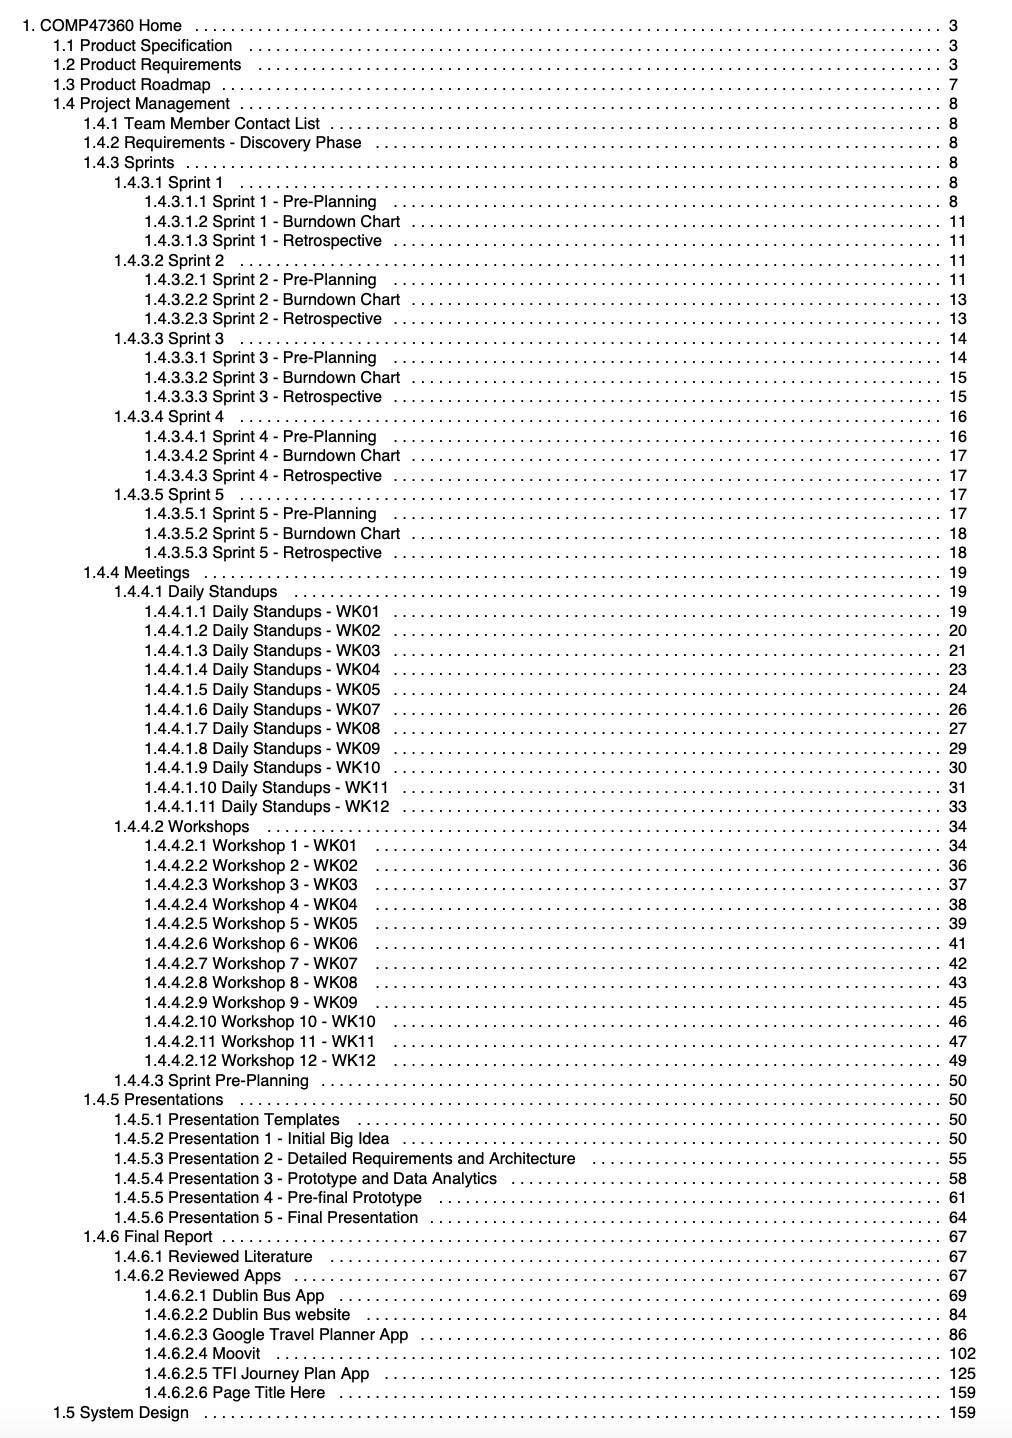
\includegraphics[width=0.4\textwidth]{figures/3_1_Confluence_1.png}
    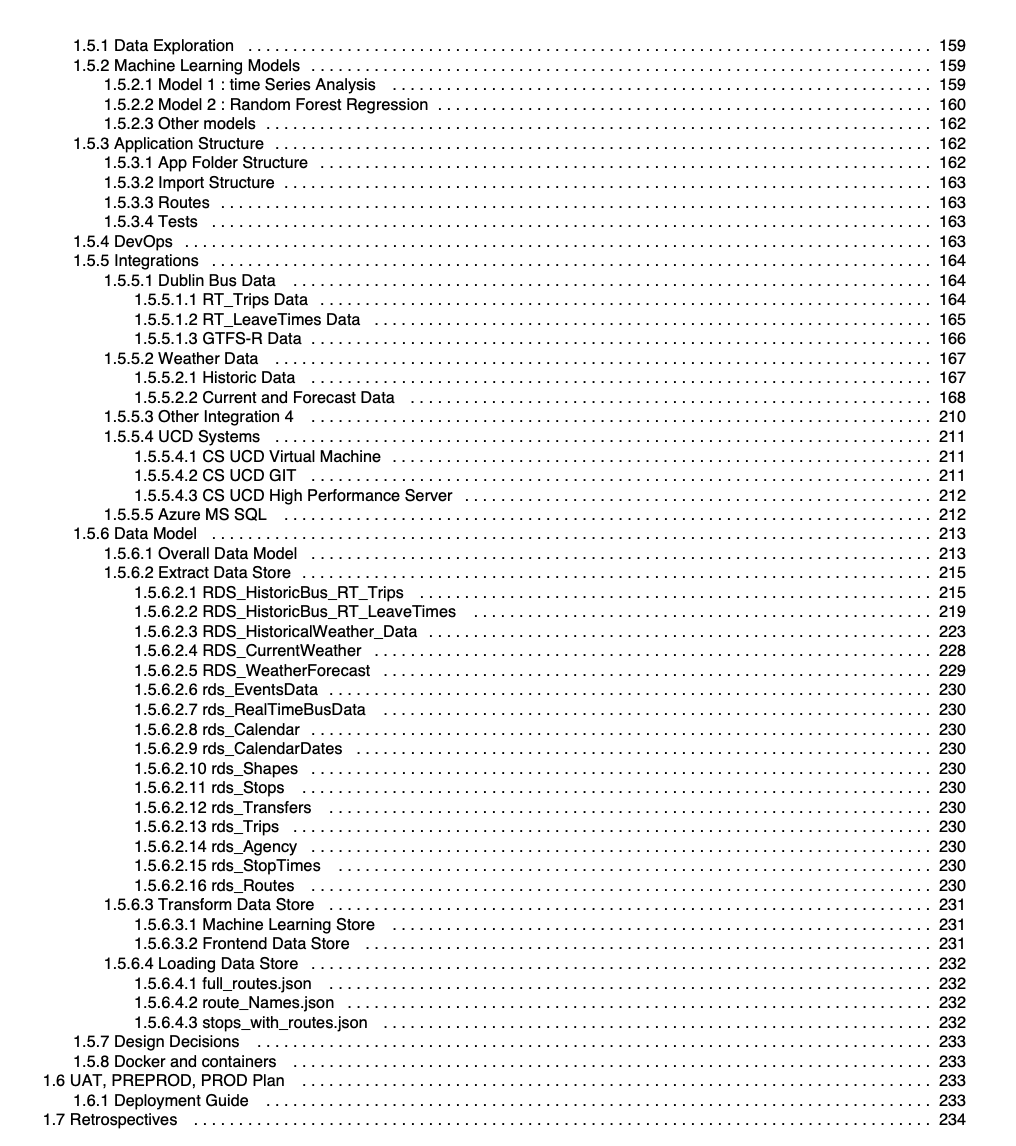
\includegraphics[width=0.4\textwidth]{figures/3_1_Confluence_2.png}
    \caption{Confluence Page Structure}
    \label{fig:ConfluenceOverview}
\end{figure}

As the project development occurred while the COVID19 pandemic was on-going \cite{COVID19}, remote collaboration was a key element in the team's approach to development of the application. Discord was the primary means of communication among the team, with Zoom used for daily stand-ups, mentor meetings, and team presentations. The key meetings which were organised regularly over the course of the project consisted of a daily stand-up occurring on Zoom at $5$:$20$pm which charted work completed in the prior day, work-in-progress, and any blockers encountered; pre-presentation meetings which occurred on Tuesdays prior to presentations for the purpose of assembling a presentation while also serving as a sprint retrospective and sprint pre-planning meeting where ways of working were reviewed and epics and tasks were planned for the next sprint; and mentor meetings where we reviewed our progress with a project mentor.

Github was used for version control of our application. Separate repositories were maintained for the Docker Container, Flask App, and Vue components. A team organisation was created within Github to house these repositories, and each repository maintained what was predominantly a Central Repository Structure where changes were tested locally and then pushed to the main branch \cite{CentralRepository}.

In the initial phase of the project, the team initially loosely stuck to the roles distributed at the beginning of the project:
\begin{itemize}
    \item Daniel - Code Lead
    \item Turlough - Coordination Lead
    \item Adam - Customer Lead
    \item Danning - Maintenance Lead
\end{itemize}
As the first sprint ended and the need for specialisation increased, the team predominantly specialised into the following roles based on a combination of personal preference and prior experience:
\begin{itemize}
    \item Daniel - Front-end Developer - Preference and prior development experience
    \item Turlough - Full-stack Developer - Prior front-end experience and interest in back-end development.
    \item Adam - Back-end Developer - Preference and prior development experience
    \item Danning - Data Analyst - Preference and undergraduate degree in Mathematics.
\end{itemize}

In the following sections we will broadly detail the high-level overview of each sprint completed.

\section{Sprint Overview}
Here we will talk about the details of the sprints, and how the sprints developed.

\subsection{Sprint 1}

It was decided to use the first sprint as a discovery phase in-line with best practices for the implementation of Agile projects \cite{GOV} to research the technologies which best suited the development goals and the key user requirements by analysing existing solutions. 

Different data sources were explored for the historic weather data including MET Eireann \cite{MET} and OpenWeatherMap \cite{OpenWeatherMap}, with the team ultimately choosing OpenWeatherMap due to familiarity, available features, and alignment with the current weather schema. Sources of data for bus occupancy and LeapCard data were explored but difficulty in the acquisition of historic and current data proved a key challenge for the team.

Docker, Flask, Azure, Github, the UCD Virtual Machine, and Vue were chosen as our key technologies during this sprint after research into the advantages and disadvantages of these technologies compared to competing technologies, and a set of initial user requirements were established after the examination of existing offerings.

The project management tools of Jira and Confluence were chosen and a structure established early to allow for immediate creation of tasks and documentation of the initial data and technical exploration.

\subsection{Sprint 2}
Following the sprint 1 retrospective, daily stand-ups were implemented from sprint 2 on-wards to allow for a greater degree of coordination among the team. The key goals of sprint two involved the creation of a skeleton application and continued data exploration.

Analysing the National Transport Agency (NTA) data set from 2018 which contains details of overall journey times and stop times became a key priority in assessing the feasibility of user requirements. Due to the high memory requirements of working with the stops data-set, we explored using a MySQL database to analyse these files but elected to use Python's Dask that can be utilized by the primary memory (RAM) rather than hard-disk space to avoid potential memory issues from using a shared drive.

Initial workflows for data exploration were created involving the creation of generalised methods for data ingestion, data cleansing, feature pairing, and visualisation to allow for rapid examination of new data sources. The current weather data schema for Dublin Bus was acquired and analysed within this sprint. 

An ER model of all elements within our data set and their relations was developed as featured, in \ref{fig:ERDiagram}, to summarise this information and outline a potential back-end architecture both to guide our application's development and to better identify how the data sources related to one another following the principle that data modelling should be completed early in project development \cite{DataModel}.
\begin{figure}[!htb]
    \centering
    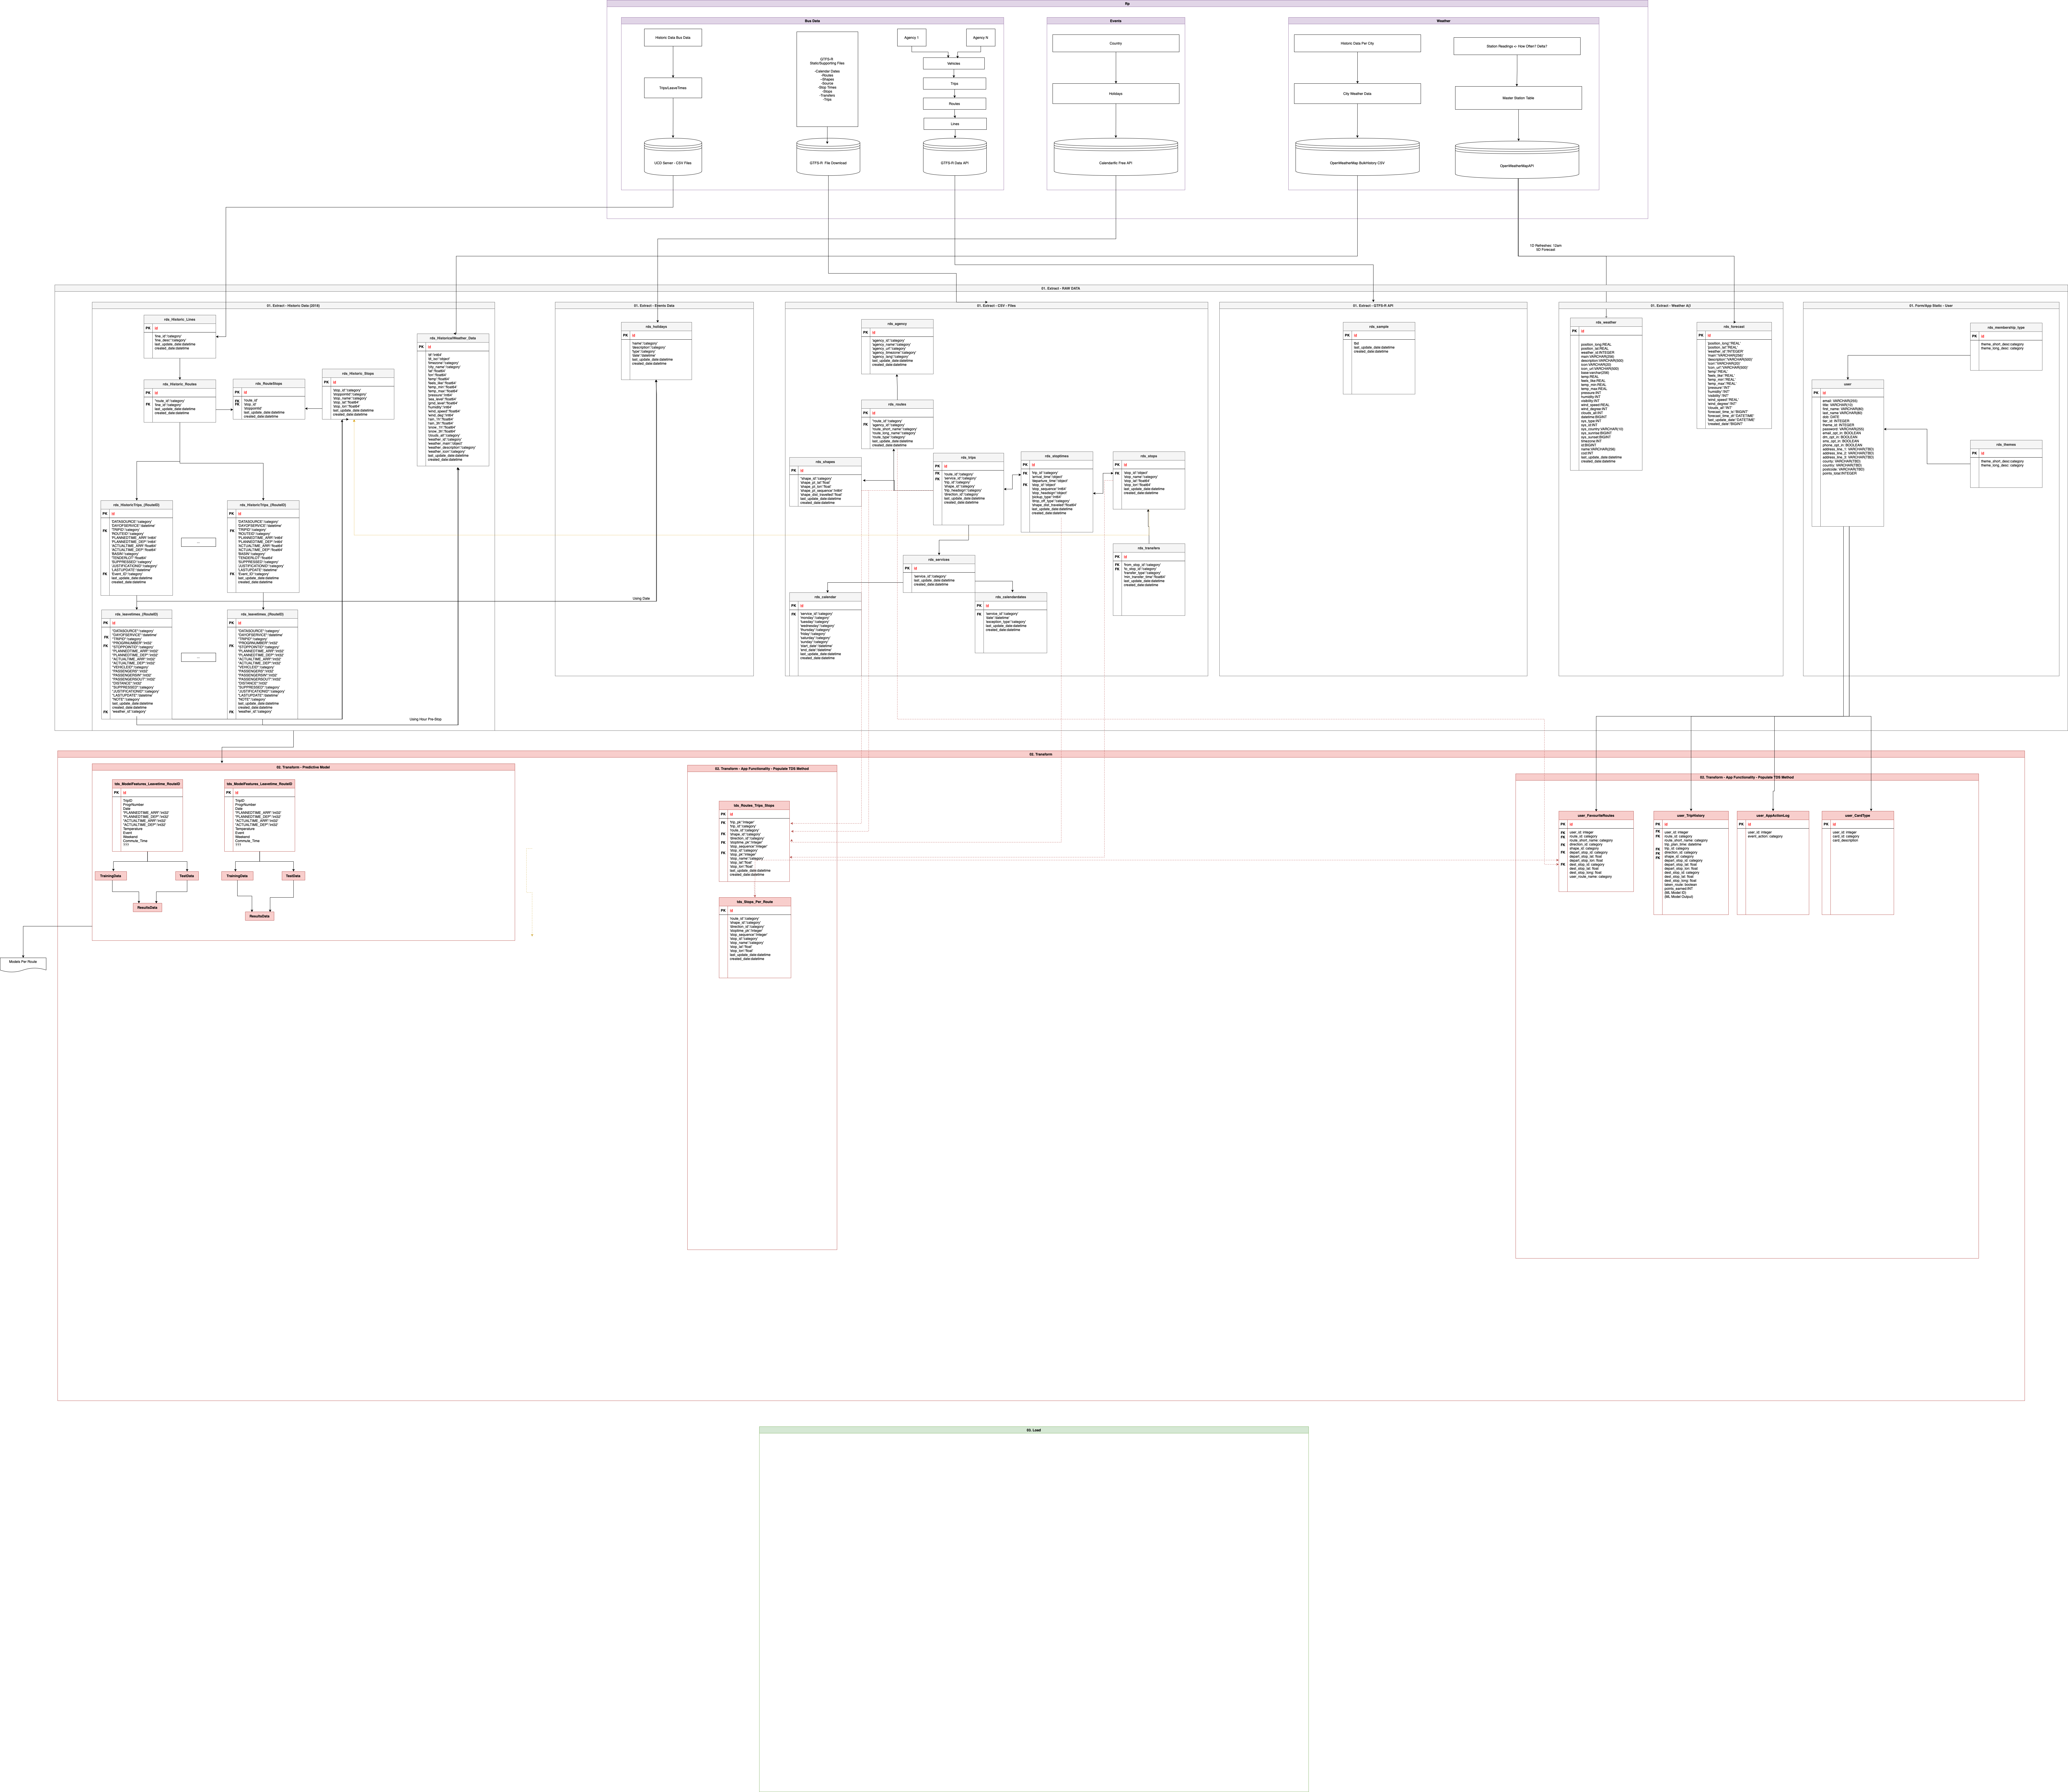
\includegraphics[width=0.95\textwidth]{figures/FinalER.png}
    \caption{The envisioned ER diagram}
    \label{fig:ERDiagram}
\end{figure}

Finally the initial application was established with early work completed in creating a structure of our application for front-end focused features.

\subsection{Sprint 3}
The third sprint focused on the development of the machine learning models, and incorporating these models into the application. Methods for data retrieval, weather features, and user login features were also incorporated and the team narrowed our possible innovative features down to a points system, admin functionality, and a business intelligence dashboard.

\subsection{Sprint 4}
The fourth sprint primarily involved honing in on which innovative feature the team would incorporate and initial testing of various components of the application to determine the optimal use of the remaining development time. The development team decided to continue the development of the user-focused features and completed general bug-fixes in the application, while beginning some of the documentation process.

\subsection{Sprint 5}
The fifth sprint involved closing out the extended features and bug fixes. As the team had deployed our application continuously throughout the project, it was possible to focus on implementing features and bug-fixes until late in sprint five at which point attention focused on the report and final presentation.
\chapter{\label{chapter4}Technical Approach}
\section{System architecture and technical stack}
The technical stack implemented was as follows
\begin{itemize}
    \item Vue and Vuetify as the front-end
    \item Flask serving as the back-end.
    \item Apache acting as the web-server and communicating with Flask via WSGI.
    \item Docker encapsulating all of the above in a deployable container.
    \item A remote Azure MSSQL database.
\end{itemize}

The above architecture details encapsulate some of the key points prioritised early in development: chiefly, that our development environments should match production as close as possible. Docker serves this purposes, allowing for (nearly) identical virtualised setups on both developer and production environments. The only architectural difference between the two is HTTPS setup; local development mandated a self-signed HTTPS cert, whereas production is authorised with a genuine cert via Let's Encrypt.

The Azure MSSQL database was accessed via Flask using SQLAlchemy and an associated MSSQL connection plugin. A remote SQL database was chosen out of concerns for potential limitations in disk space present on the provided UCD Virtual Machine server instance; in contrast, Azure provides generous storage space.

\begin{figure}[!htb]
    \centering
    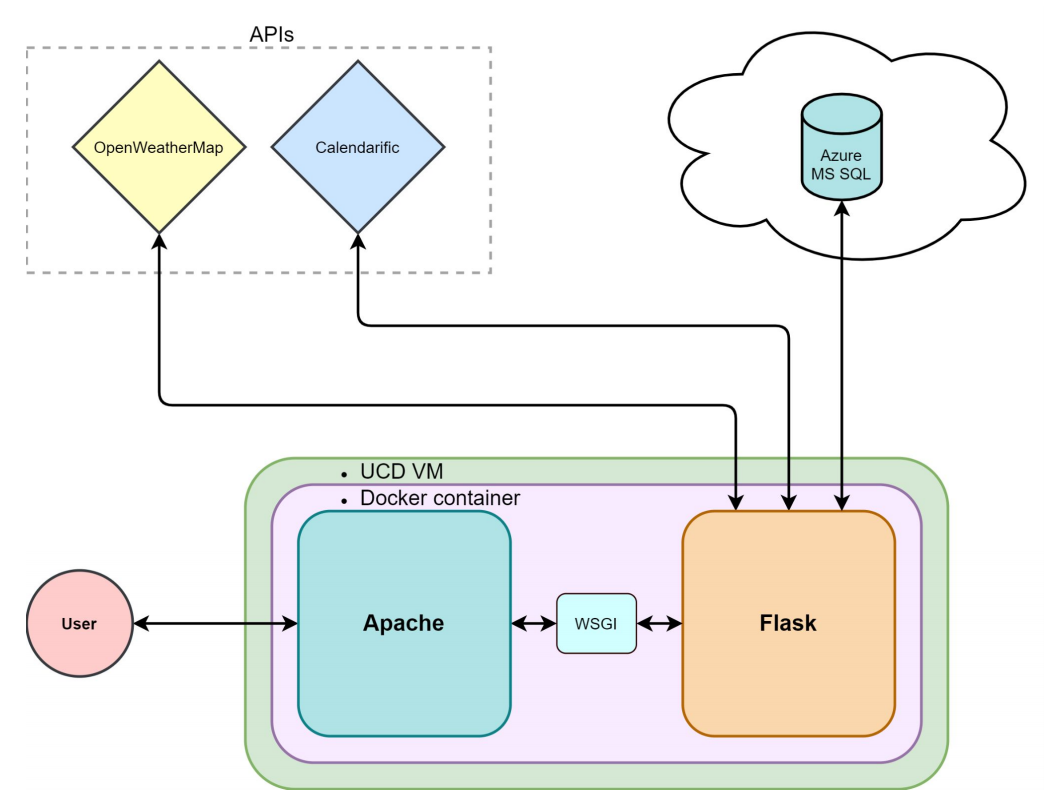
\includegraphics[width=0.7\textwidth]{figures/ArchitectureOverview.PNG}
    \caption{Architecture overview}
    \label{fig:ArchOverview}
\end{figure}

The technical details pertaining to the selection and development of the above stack has been split into Front-end, Back-end, and Data Analytics. Fluid development and communication between these three main technological areas was crucial for the successful development and deployment of the web application.

\section{Front-end}
\subsubsection{Vue and Vuetify}
A core tenet of the front-end development approach in the early planning phases was to create an aesthetically pleasing, functional, and responsive front-end environment for our targeted user demographic. These criteria are well served by front-end JavaScript frameworks. There are a myriad of such frameworks available; as such, it was necessary to research and select the most suitable one for the project purpose. The key frameworks considered were Angular, React, and Vue. Many of these frameworks have dedicated front-end component frameworks that are designed around delivering a certain visual style; as such, it was necessary to consider both the underlying framework (Vue, Angular, React), and its associated ecosystem (BootstrapVue, Angular Material, etc.). 

Vue was selected as the underlying framework of choice due to its focus on developer friendliness and ease of use in contrast to the more established but less beginner-friendly React and less-liked Angular \cite{SO-SurveyFrontEnd}. In selecting an accompanying component library, the Vuetify front-end component framework was chosen; Vuetify offers a consistent visual style of components and interface elements based on the Material Design visual standard originally created by Google \cite{MD}.

%Vue facilitates development through the built-in development server, which can be launched via the command "npm run serve", and changes made to files will refresh the server instantly allowing for immediate iteration on features/bug fixes.

\subsubsection{Vue Router and Views}
For the purposes of user navigation, the optional but tightly-integrated Vue Router plugin was set up and configured for the project. This allows for seamless in-page content loading and navigation, allowing the front-end to be structured in so-called "View" files that are dynamically loaded into the main page content area when a user navigates around the front-end using the configured and presented Vue Router "Routes", which can be functionally considered as equal to conventional hyperlinks. This encourages a modularised file structure as each distinct page (Login, Map, Profile etc.) is its own Vue file, and linking to this "View" is done with Vue Router "Routes". 

\begin{figure}[!htb]
    \centering
    
\includegraphics[width=0.4\textwidth]{figures/vueRouterViews.PNG}
    \caption{The "Views" for Vue Router}
    \label{fig:RouterViews}
\end{figure}

\subsubsection{URL query parameters}
Vue Router also enabled the URL query parameter operations that formed the backbone of the shareable links feature; it allows for encoding any desired parameters in the user's address bar, and likewise a user landing on the page with a pre-configured URL can have said parameters read and automatically applied to the site. For each query that the team desired to encode in the URL, an associated function was written, which would "push" the query parameter to the user's URL. These functions were called whenever the user modified said variable; as such, the URL updates live with any changes the user inputs. This is visible in figure \ref{fig:QueryURL}.

\begin{figure}[!htb]
    \centering
    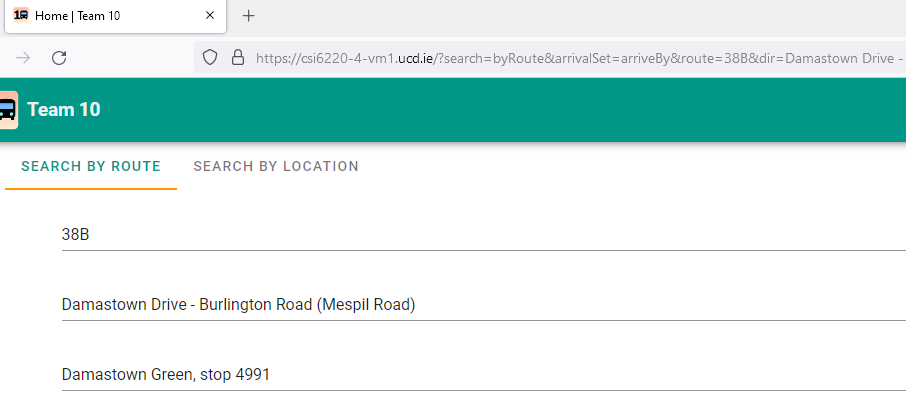
\includegraphics[width=0.7\textwidth]{figures/URLParams.PNG}
    \caption{Query parameters reacting to inputs}
    \label{fig:QueryURL}
\end{figure}

To actually utilise these query parameters, a Vue Watch option was written for the route query parameters. In short, Watch functions will continuously monitor a specified Vue data element (in this case, the user's URL and associated query parameters) and perform some function when said element changes. This means that users first accessing the site will trigger the Watch logic that modifies the page contents to match their URL's associated queries.

While a shareable link is a feature in its own right, this feature also enabled our saved routes functionality; when a user saves a route, our database stores the individual elements of the user's choice (route, direction, start/end stop etc.). In retrieving this data, the application crafts a hyperlink using the previously described method and presents this as "retrieving" a stored route.

\subsubsection{Components}
One of the underlying principles of Vue is the creation and use of components. These are reusable HTML, JavaScript and Vue objects that can be added to any part of any other Vue file via the equivalent of an import statement. This enforces some basic principles of the Vue development concepts: that repeating sections or elements of a page should be split out into components; that data should flow from parent document to component; and that components should be reused as often as possible. 

\begin{figure}[!htb]
    \centering
    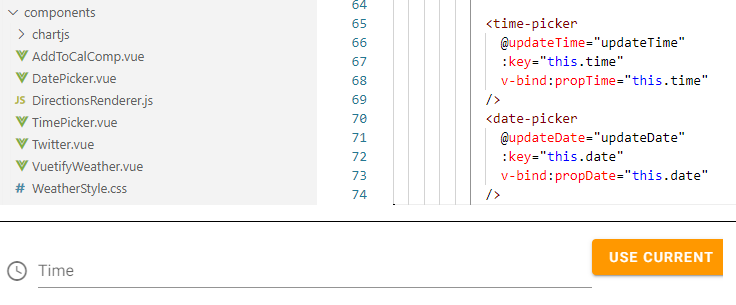
\includegraphics[width=0.7\textwidth]{figures/componentFinal.png}
    \caption{Component example}
    \label{fig:ComponentExample}
\end{figure}

An example of the component system is shown in figure \ref{fig:ComponentExample}. On the upper left is the component folder structure of the project; on the right, we see the process of declaring an instance of the component to be included in "Maps.vue"; and finally at the bottom of the image, we see the rendered time picker component itself ("TimePicker.vue"). 

\subsubsection{Open Source Community Software}
Leveraging community and open-source projects underpins much of modern software development, across commercial and hobbyist development alike. In undertaking this project, we sought to enhance our application with existing solutions where feasible \cite{Optaros}.

\href{https://www.npmjs.com/package/vue2-google-maps}{vue2-google-maps} performed the role of a Vue-based implementation of the Google Maps API. It effectively wraps the Google Maps API and functionalities in a Vue-ready state, allowing for general Vue-centric approaches like data binding and updating, while also providing other components, such as the Auto-complete Search API wrapper; this is the Google-based locations auto-complete search bar which appears in the "Search by Location" tab for user origin and destination searching. Further functionality was added to the map proper with a handmade component, "DirectionsRenderer.js", which serves to draw a Google Maps Directions route on the map, and clear it when desired. %This is shown in figure \ref{fig:DirectionsExample}.

%\begin{figure}[!htb]
%    \centering
%    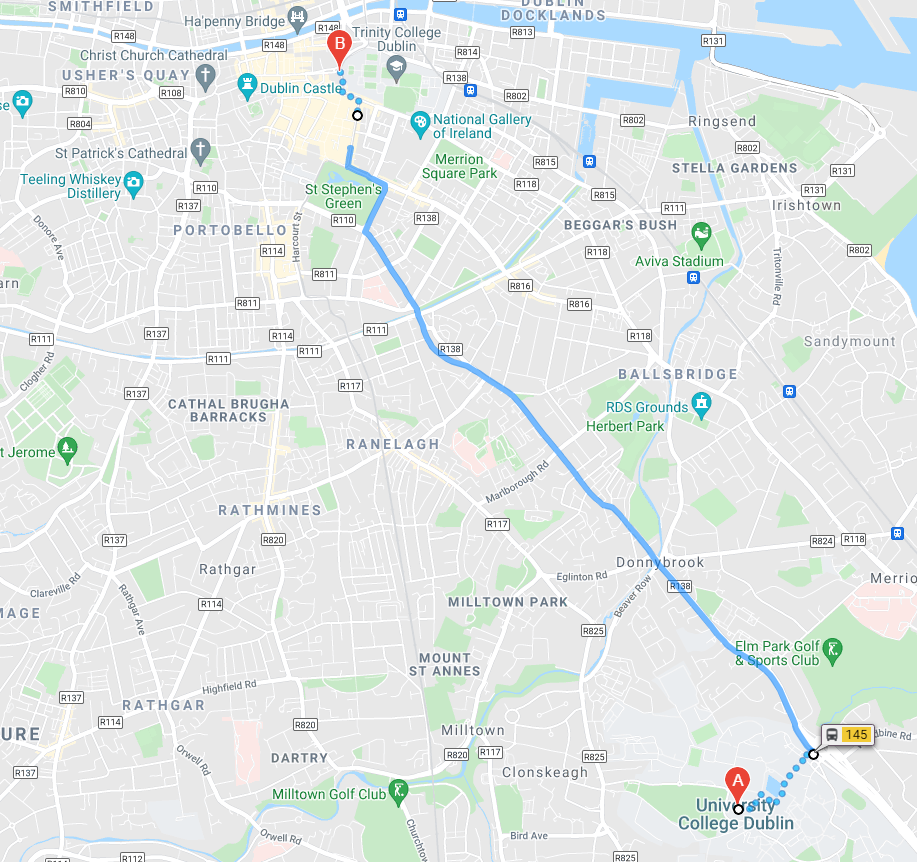
\includegraphics[width=0.5\textwidth]{figures/directionsRenderer.PNG}
%    \caption{DirectionsRenderer.js drawing a route}
%    \label{fig:DirectionsExample}
%\end{figure}

To achieve the desired "add to calendar" functionality, the team leveraged the \href{https://www.npmjs.com/package/vue-add-to-calendar}{vue-add-to-calendar} package to generate clickable links to add the desired event to a user's Google, Microsoft, or Office365 calendar which involved installing the application locally for installation. vue-add-to-calendar is provided under the MIT license. 

In creating the weather widget functionality present on our developed web application, \href{https://github.com/dipu-bd/vue-weather-widget}{Vue Weather Widget} was forked and heavily modified. It was necessary to heavily modify this project as in its original state, it directly queried the OpenWeatherMap API for every page load. As the team was only on the free tier of said API, there was concern regarding OpenWeatherMap's API limits; additionally, this API was already being queried on a timer by the Flask instance to write current weather data and forecast data to an Azure table for future analysis. It was decided to modify the underlying functionality of the weather widget to instead query one of the Flask routes, which would provide a cached response of the latest weather as stored in the Azure database. 

After this technical rewrite, it was also deemed desirable to provide a visualisation of the temperature for the next 48 hours. Vue Weather Widget did not provide this functionality; as such, it was added by the team via ApexCharts, an open-source data visualisation library that proved a joy to work with.

It was then deemed desirable to migrate Vue Weather Widget and the newly-added chart visualisation feature into a single, streamlined Vue component, and not as an installable Vue module. This was carried out, and the forked repository was marked as defunct, with all future work now being carried out on "VuetifyWeather.vue". %The final result is visible in figure \ref{fig:weatherExample}

%\begin{figure}[!htb]
%    \centering
%    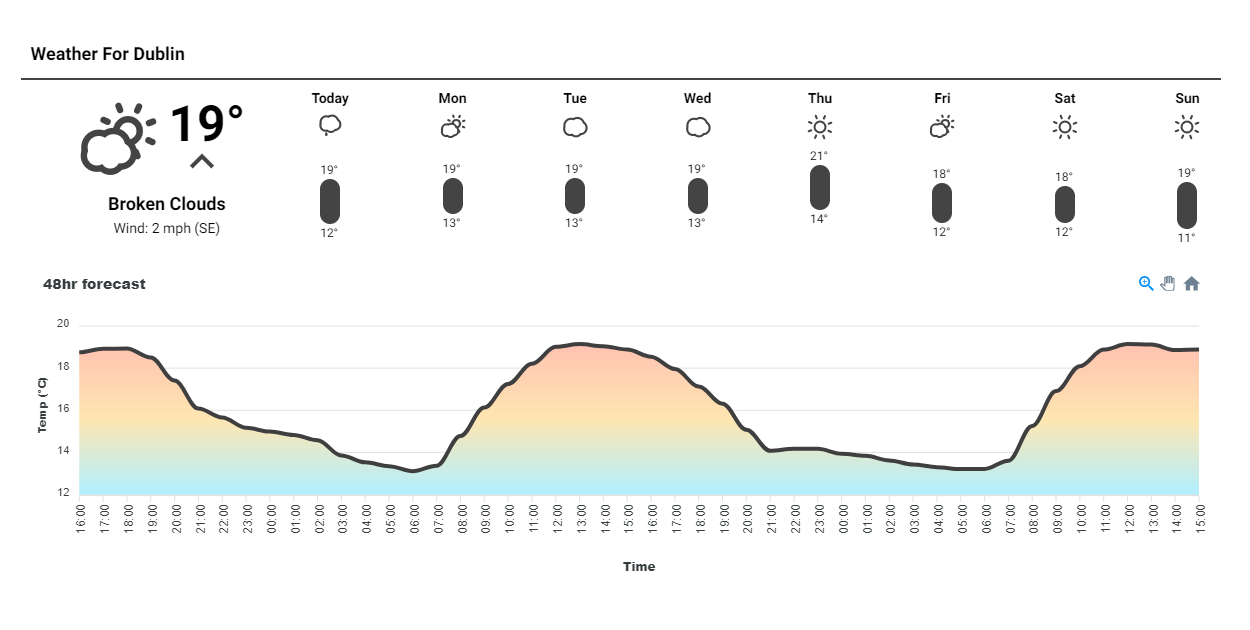
\includegraphics[width=0.7\textwidth]{figures/Weather.PNG}
%    \caption{Final weather view}
%    \label{fig:weatherExample}
%\end{figure}

\subsubsection{User login and dynamic U.I}
A user login feature was developed across both the front-end and back-end of this project, facilitating user account creation, deletion, and logging-in. Data pertaining to the functionality of the site can be saved to a logged-in user's account details on our Azure database. The technical details for the login system are covered later on in the back-end section; however, it is important to note that the front-end responds dynamically to whether or not a user is logged in upon visiting the site. A guest user, for example, is shown different navigation links in the navbar of the site than a logged-in user; this serves to prevent users from accidentally accessing sections of the site restricted to logged-in users, such as the Profile page.

\begin{figure}[!htb]
    \centering
    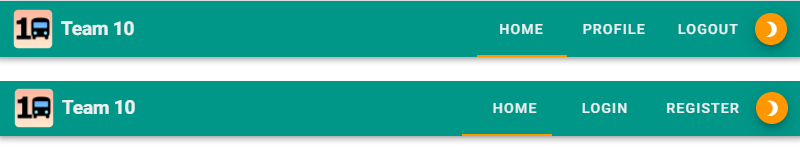
\includegraphics[width=0.7\textwidth]{figures/loggedInExample.png}
    \caption{Logged in (top) vs not (bottom) navbar}
    \label{fig:NavbarLoggedIn}
\end{figure}

It was planned that this functionality would be extended to other minor U.I elements on the page, such that anything that requires a user to be logged-in to function (saving a route; showing saved routes, etc.) would only be visible if the user was indeed logged-in. Unfortunately, these details dropped out of development scope in sight of the code freeze deadline; the responsive navbar seen in figure \ref{fig:NavbarLoggedIn} is the primary example of dynamic U.I. implemented.

%Other minor details of a dynamic U.I based on a user's logged-in status appear in the profile page, where a user is greeted with a message personalised with their name as provided during registration.

\subsubsection{Forms, GETs, and POSTs}
For the purposes of passing data from the front-end to the back-end, POST requests were used almost exclusively. Although in recent years other paradigms of data transfer between client and server have become mainstream (WebSockets being a prime example), for the purposes of this project, aspects such as registration forms or login pages were handled more than adequately via HTTP using formdata JavaScript objects. It is in this way that the front-end communicates with the back-end to e.g retrieve a user's saved routes based on the currently logged-in user's user ID, to then populate the front-end list of clickable URLs to a saved route.

%For example, to enable the "saved routes" feature, the front-end sends a POST request message to the back-end route "/profile/returnSavedRoutes". Flask then interprets the POST data form and looks for the "userID" form field, this being the required variable for the SQL query subsequently performed to extract said saved routes data from our database, which is then returned Flask, which in turn returns this result as the HTTP response to our front-end request. This response is then parsed by the front-end into a list of clickable links that represent the user's saved routes.

Personal data is secured via HTTPS, ensuring that user details are not easily intercepted in transit when registering/logging in.
A portion of tech debt was intended to be eliminated by replacing the individual GET/POST requests with a single master HTTP GET/POST function which would accept all required inputs to make the relevant GET/POST requests. This was deemed infeasible in the time remaining for the project and as such, each GET or POST request to a specific endpoint has its own relevant function.

\subsubsection{Twitter integration}
Twitter was integrated using Twitter's \href{https://developer.twitter.com/en/docs/twitter-for-websites/embedded-tweets/overview}{developer-friendly embed page}. By inputting the page for Dublin Bus' twitter account an embedded code snippet is generated which was then integrated into the application.

\subsubsection{Dark mode}
Dark mode is a native functionality in Vuetify; enabling this functionality simply required displaying some UI element (a button, link, etc.) which would trigger the built-in switch. It was necessary, however, to define some of the theme colours for dark mode, due to text legibility issues.

Using vue2-google-maps it was possible to dynamically modify the main maps' colour theme when switching to/from dark mode. These themes are defined in "mapStyles.json". %See figure \ref{fig:DarkmodeExample}.

%\begin{figure}[!htb]
%    \centering
%    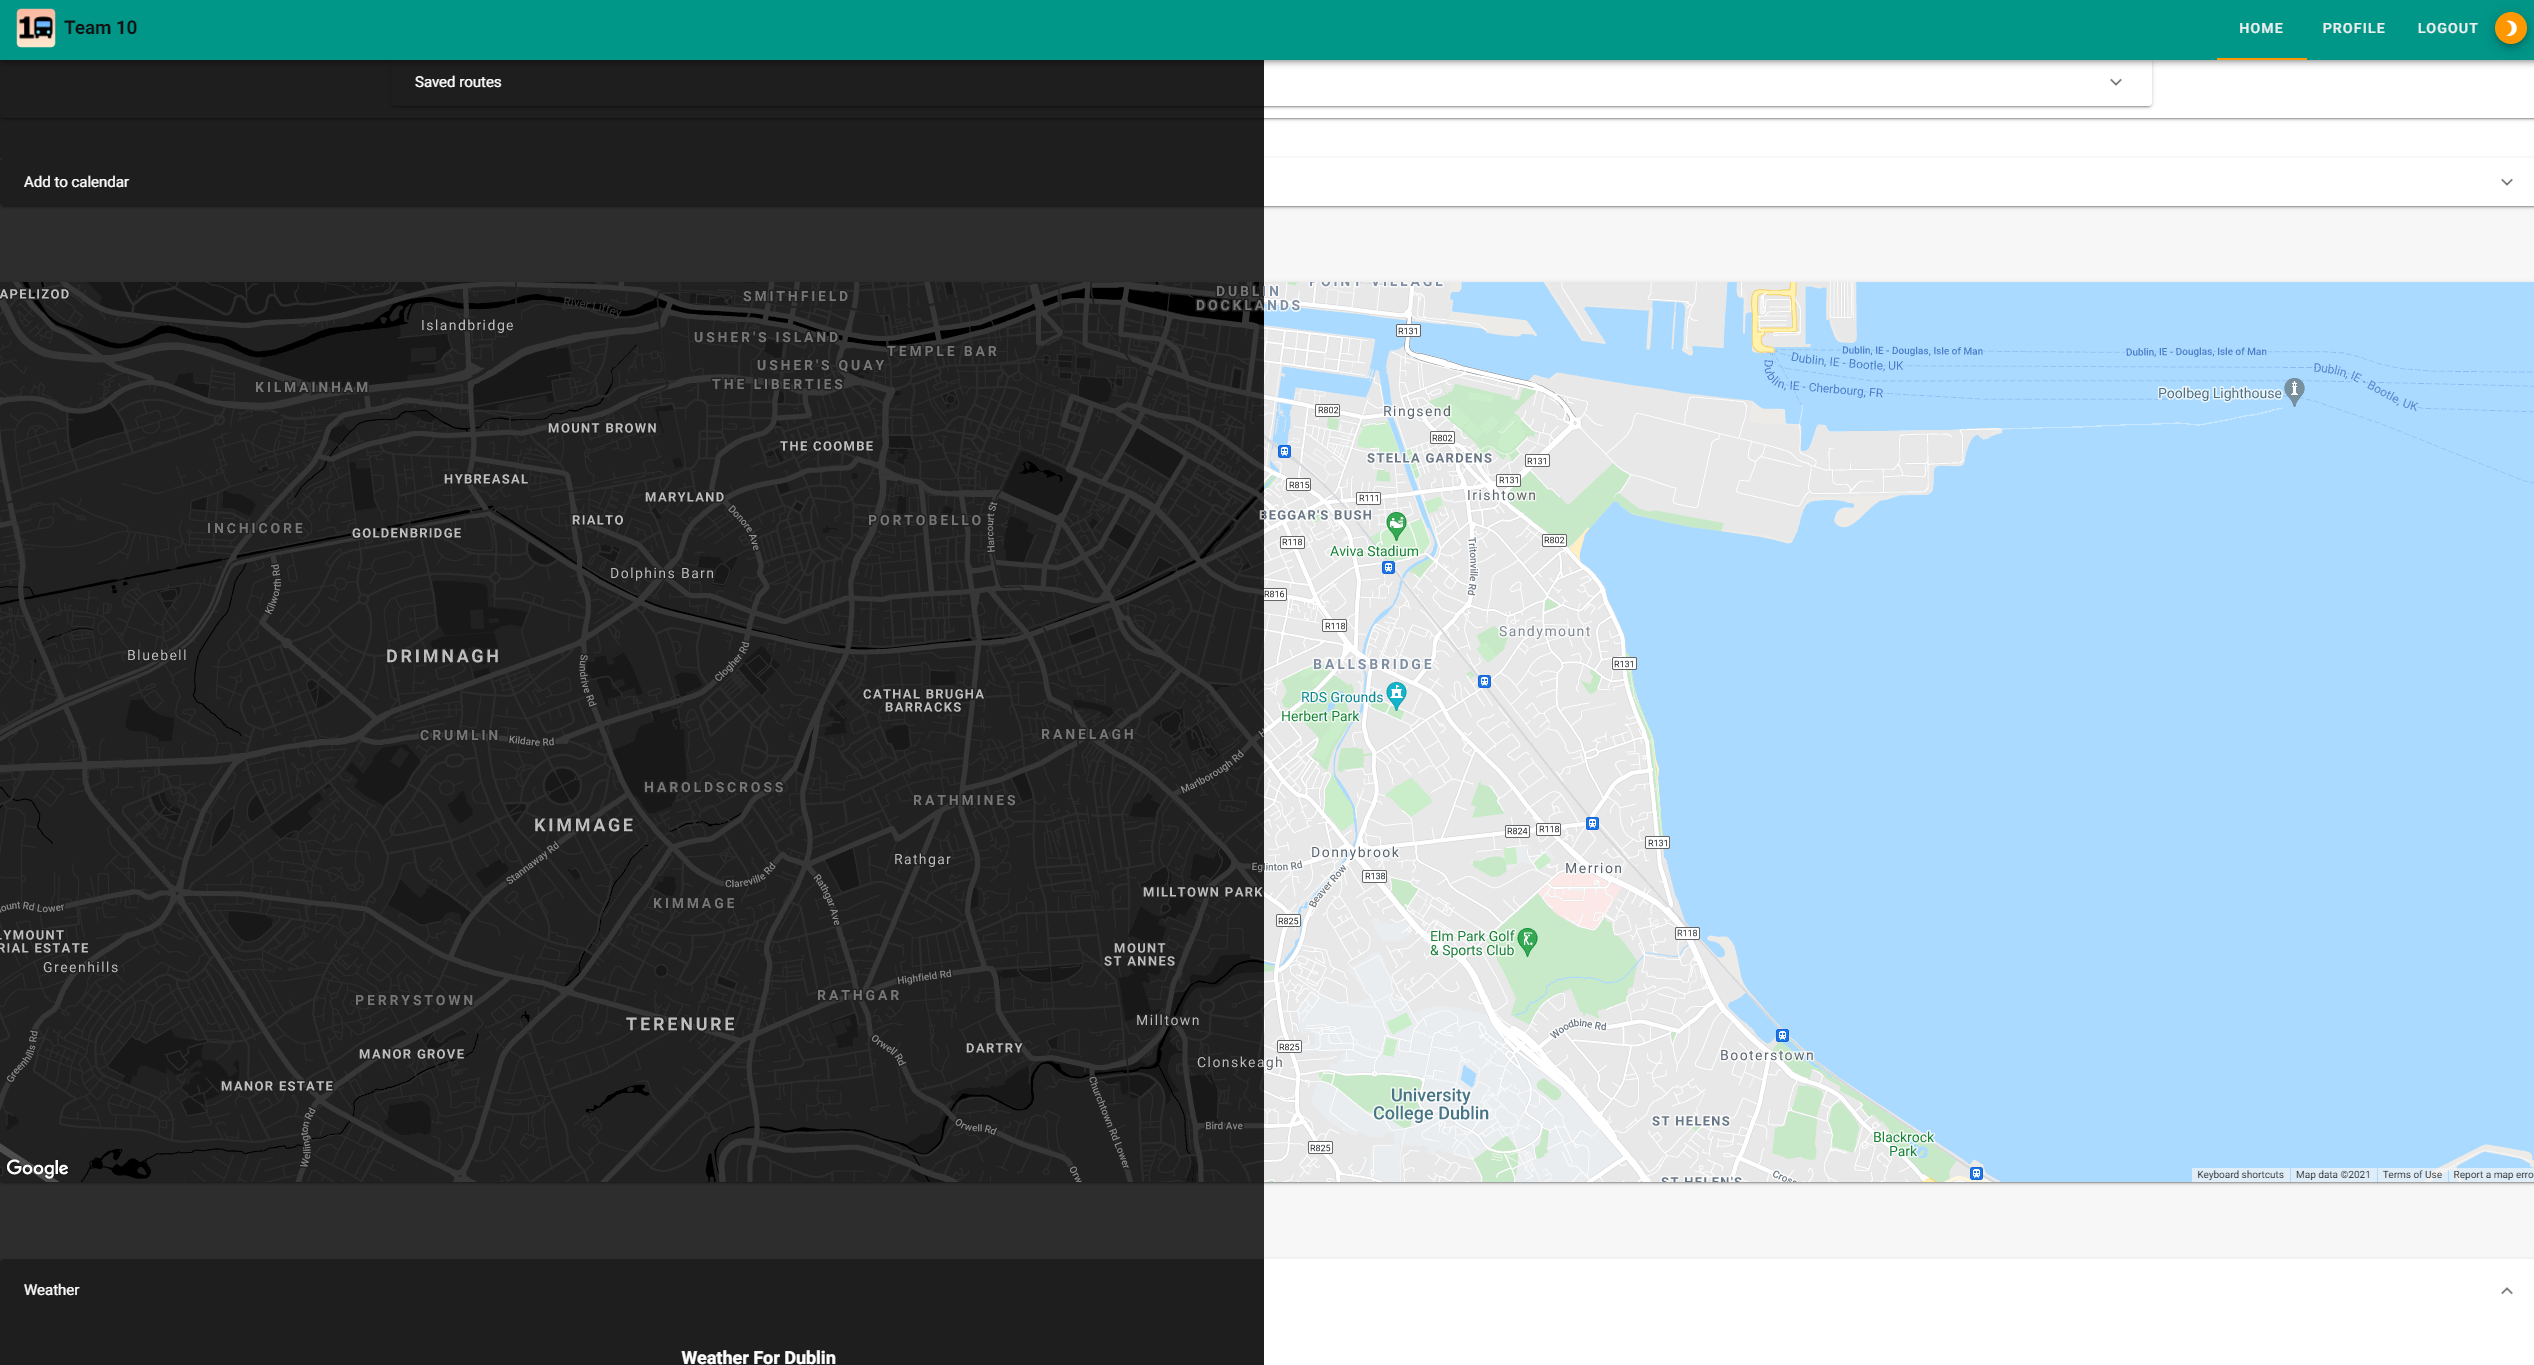
\includegraphics[width=0.6\textwidth]{figures/darkmode.png}
%    \caption{Darkmode propagates to the map}
%    \label{fig:DarkmodeExample}
%\end{figure}

\newpage

\section{Back-End}
The web application runs on a Flask back-end framework. Flask is a light-weight and highly modular back-end framework allowing for more flexible design patterns, and has become increasingly popular as a Python back-end, but one which requires greater developer effort to build some of the application features which Django provides \cite{WhyFlask}. Django is a fully-featured Model-View-Controller back-end framework used across industries by large organisations including National Geographic, Instragram, Disqus, and EY. It's a flexible and scaleable back-end framework which comes fully-shipped with out-of-the-box solutions for a variety of development tasks included with the aim of helping developers create applications quickly \cite{WhyDjango}.

A key initial decision in the project was in determining which back-end framework was most suitable for the project goals and timeline which the team faced. While Django had advantages in enforcing best development practices through its design structure, and contained out-of-the-box solutions for the user system which was planned on being implemented, the team determined that Flask would be most suitable for the application. Due to the low volume of expected users in the application negating the need for a highly scaleable solution, and due to the overhead of learning Django while the team was already familiar with developing a Flask application through experience in the COMP30830 module, it was determined that Flask would be sufficient for the needs of the application and any additional development time required in incorporating some of the aspects which Django provides would be offset by the familiarity which was already present from using Flask while also having the advantage of being lightweight.

Azure is used as a data storage tool within the application to store Dublin Bus data and weather data. This was chosen over alternatives such as AWS and MySQL due to the free data storage provision on the student license, and a need to minimise storage on the UCD Virtual Machine. Front-end inputs are passed through routes and if relevant stored in the Azure database. 

\subsection{Why Docker?}

With the volume of back-end and front-end tools in use, aligning team members' technical set-up was a key initial goal. Docker is a system which allows containerised instances of software stacks. Containers are microcosms of operating systems and software configurations; Docker containers leverage the widespread availability of virtualisation technology in modern CPUs to run instances of other operating systems from within the user's base OS, and each of these instances is referred to as a “container”. A Dockerfile is used to establish the container, and to activate this container a user “builds” the dockerfile out to a full container which is then rebuilt upon changes; typically in the setup one pulls an image of an operating system, and specifies what commands Docker should then run such as the installation of Python. As Docker allows one to map internal ports in each container to actual ports on the real system, a web-server running in a docker container might think it’s running on ports 80 and 443, but it’s actually accessible on the machine on ports 101 and 5665, as one can tell Docker to expose those internal ports on those external ports, allowing the team to run a node-express-nginx stack in one container directly adjacent to a flask-wsgi-apache instance, on different external ports, allowing both containers to inter-operate on the end system when referenced with their exposed external ports.

The key benefit to Docker for the team was that once a container is defined, containers can be stopped, changed, and rebuilt rapidly. In contrast to configuring a Virtual Machine with the desired web stack, a docker container can be modified, shut down, or rolled back to a previous configuration if required, eliminating the need for backups present in a Virtual Machine.
\newpage

\section{Data Analytics}\label{DA}
Python, Jupyter Notebook, and SQL were the key technologies used for data analysis during the course of the project. Key data sets which were analysed included the Dublin Bus 2018 data, Dublin Bus's static 2021 data, OpenWeatherMap's historic and current data, and Google's API Response data.

A key challenge faced during the analysis of the historic bus data, encompassing overall journey data and individual stop data, was in the volume of data which was provided. Data on stop data for 2018 comprised 11GB presenting a key challenge in analysing the data; Pandas proved insufficient for accessing a data-set of this volume. By using a package called Dask, this large data-set was split by route allowing for standard analytic libraries and methods to be used. While SQL was considered as a solution, a key concern was that as the team was using a shared machine with other groups, the team was concerned with potential space limitations and the performance of this process over a shared drive, in addition to the need to continuously query a large data-set.

Following the splitting of the historic data, a data exploration process was developed to allow for a rapid ingestion, cleansing, and feature-pairing for new data-sets. Using this process the team was able to rapidly interpret the variety of data-sets which were encountered when this process was supplemented both with data dictionaries from the data providers and the team's data model as highlighted in chapter \ref{chapter3} and focus could be placed on methods for data cleansing and feature selection from the historic data for the machine learning model.

By creating a feature correlation graph as in figure \ref{fig:CorrelationGraph} and analysing the features which were most heavily correlated with the target feature of delay time, and supplementing this with background knowledge and the 2021 data features, the most promising features for the model were chosen as 
\begin{itemize}
    \item stop-index-number - Number of stop on Route
    \item hour - Hour of Trip
    \item minute - Minute of Trip
    \item holiday\_index - Is the month in June, July, August, December or a public holiday
    \item direction - The direction of the route
    \item humidity - The humidity
    \item rain\_1h - The rainfall in the last hour.
\end{itemize}

\begin{figure}[!htb]
    \centering
    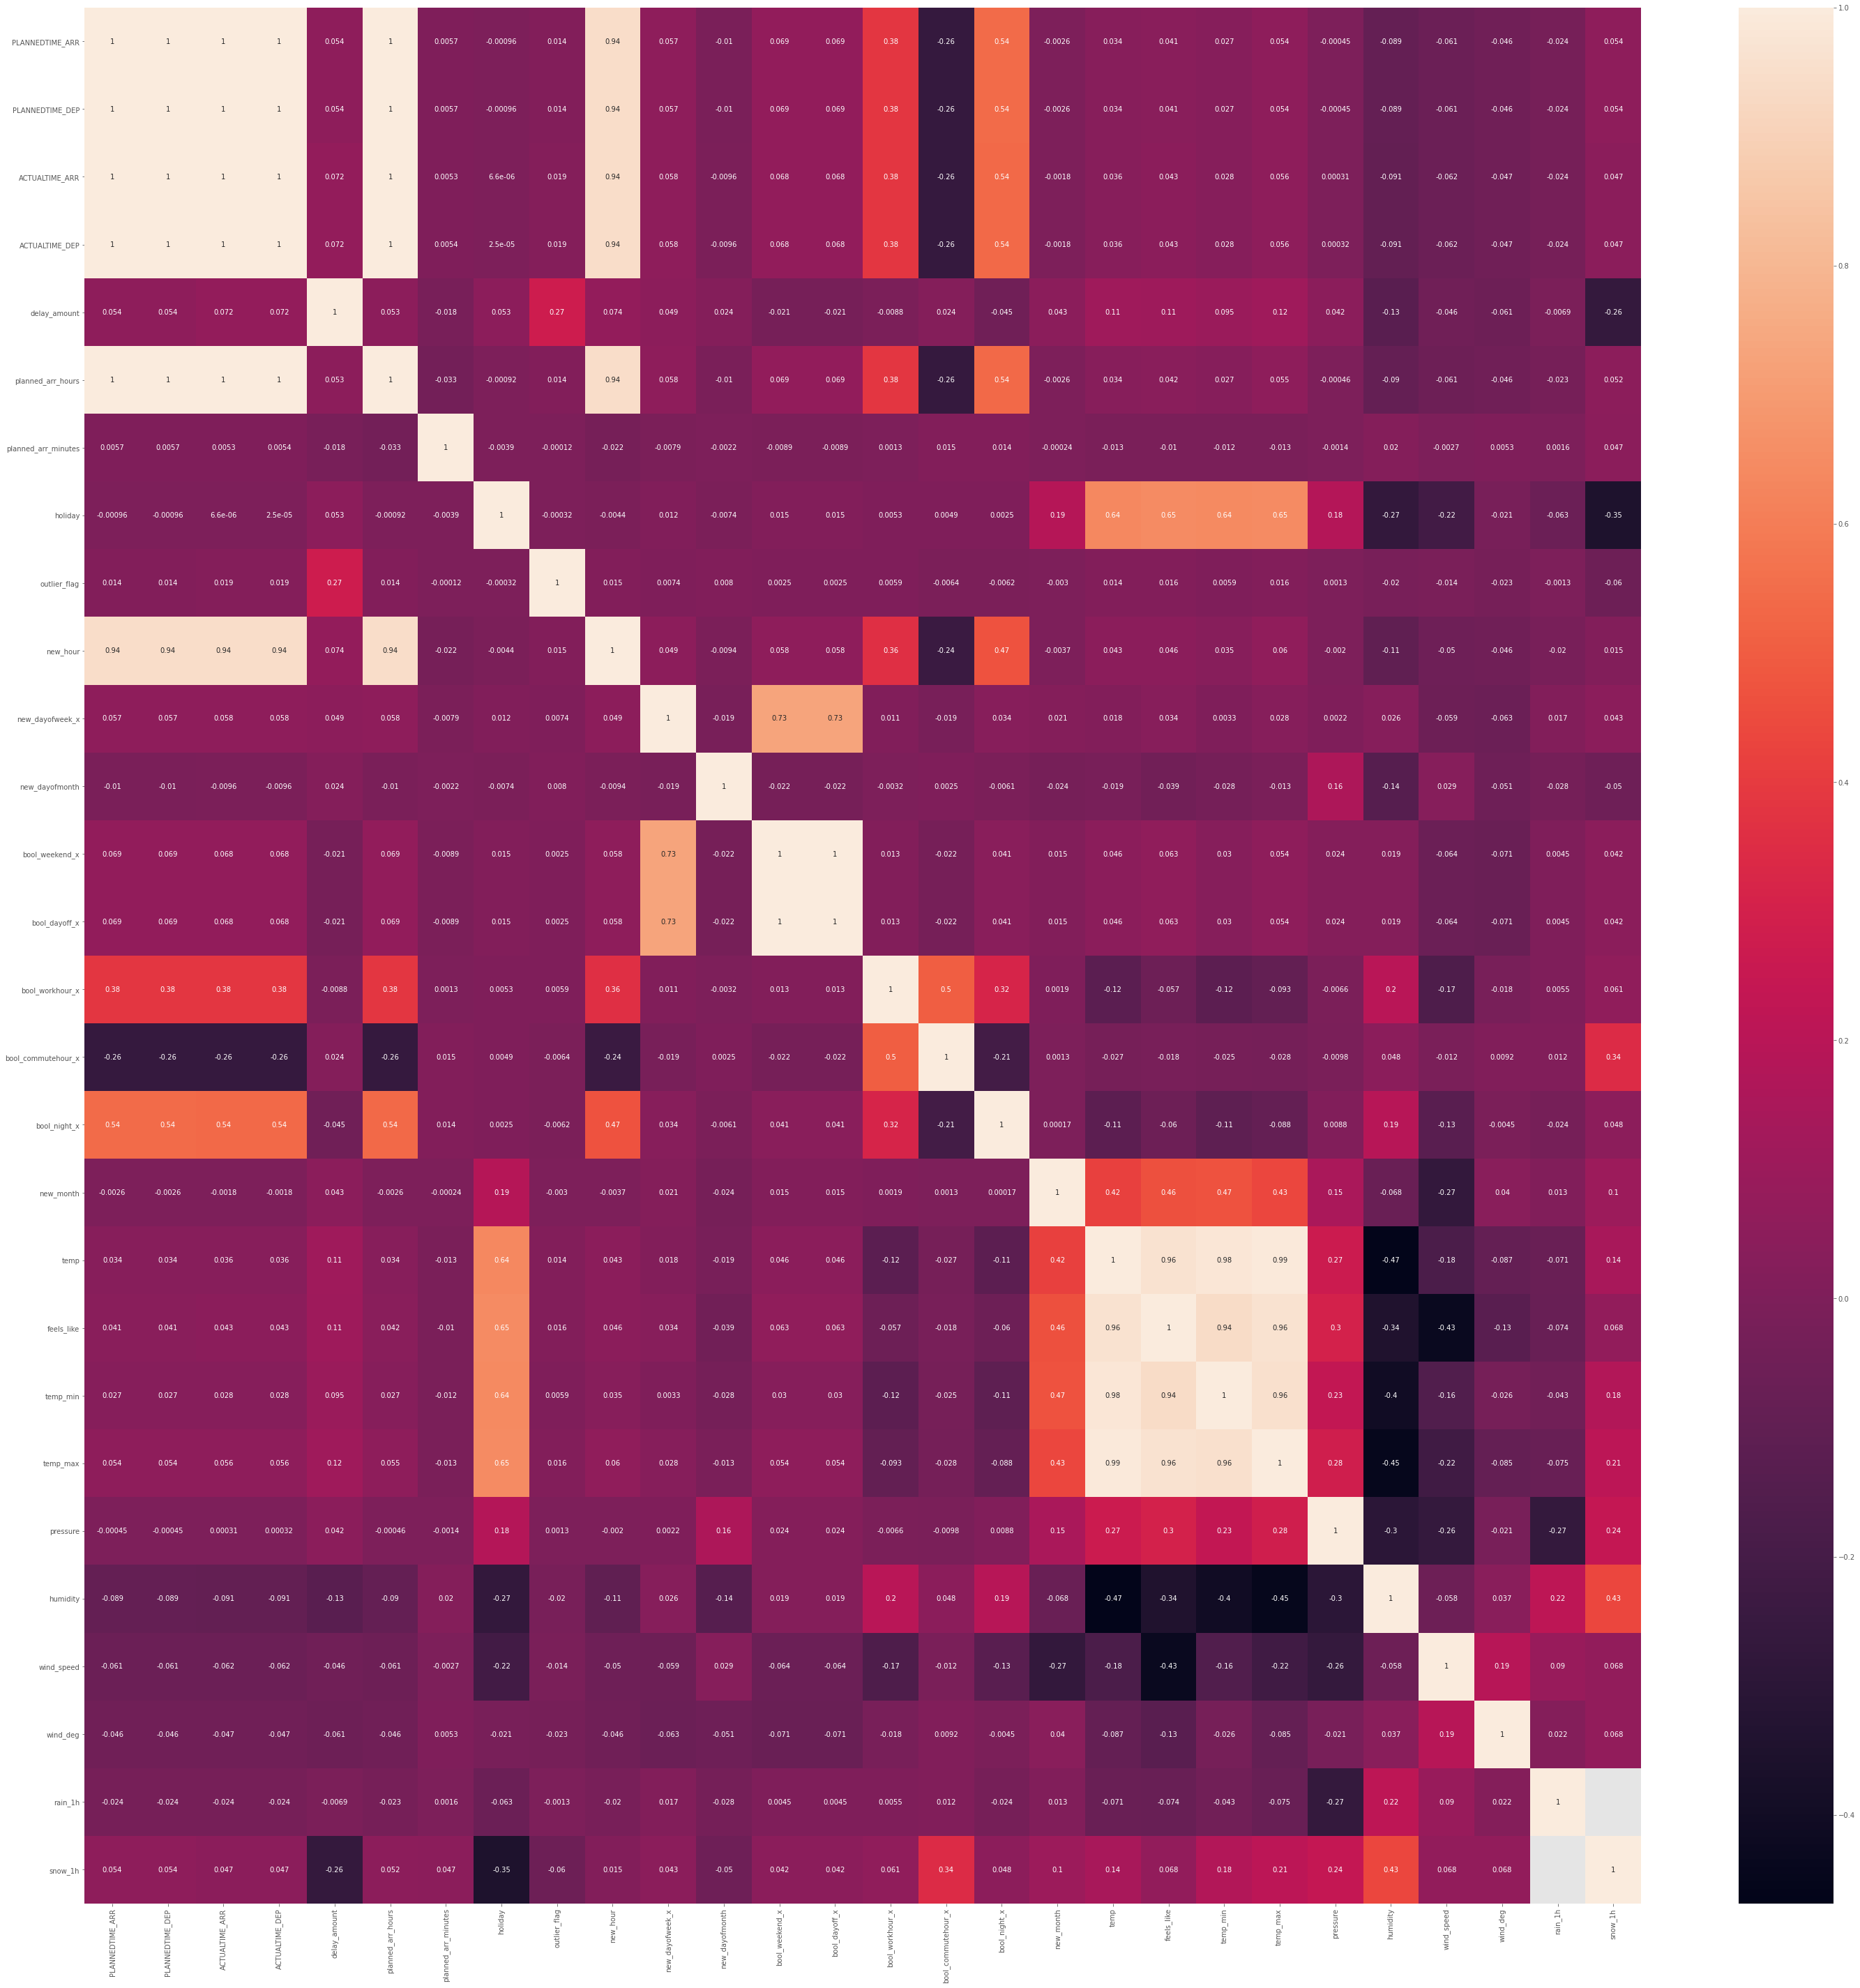
\includegraphics[width=0.85\textwidth]{figures/CorrelationGraph.png}
    \caption{A feature correlation graph for Route 102}
    \label{fig:CorrelationGraph}
\end{figure}

\subsection{Model Selection}
As the data itself can be formed into a time series using many different units of time, many different units of measures of time can be used to form the time series. Hours could be used to form a time series, but this would necessitate the construction of the entire time line on the model and using the already formed function to get the predicted values. A key issue with this is the need to assume that the data distribution for the time series will be the same each day which would require training a significant volume of time series models resulting in a significant cost in time and computational power to create and store the models. Alternatively, a time series model which incorporates the entire year could be trained, but due to the high correlation of time with delay this may lead to a high variance for each of the hours. As the time series model would take in an input for time and returns a data-point with respect to the time, the usage of historical data applied to the current date and time would result in a forecast with a very high variance. Due to these factors we decided against the use of a time series model as the variance for the prediction was too high, the model input too limited, and computational time too significant given that the models would be trained on a shared UCD server.

Linear regression and random forest were then considered due to prevalence in literature \cite{RF}, and the speed of training time which was a key consideration due to the shared nature of the UCD Virtual Machine. Two potential models were considered, the first being models based on all of the stops in Dublin that are associated with the bus network and the second was a per route model. Due to the stop volume, this approach required a large number of models, putting the server under more strain, and hence the decision was made to train models on a per route basis. After creating the models, the features chosen from the exploratory analysis were tested for both linear regression and Random Forest Regression models. These models were trained on sample routes and compared using mean absolute error (MAE) and root mean squared error (RMSE), with Random Forest resulting in the optimal balance of speed and error results as discussed in section \ref{DA-eval}. The error was calculated on a 70-30 train-test split which was split based on the date. XGBoost was considered as an approach due to high performance in Kaggle Competitions \cite{XGB}, but when combined with GridSearchCV for optimal hyperparameter tuning, the models were too time-intensive to train for a minimal improvement over Random Forest.


\chapter{\label{chapter5}Testing and Evaluation}
This section documents the development team’s testing and evaluation strategy for the application, broken down by the respective evaluation strategies for its front-end and analytics components. Performance testing of the application’s Flask back-end was limited to error-handling in functions, and as such this is a key area for future improvements.

\section{Front-end Evaluation}
The front-end of the application was evaluated by two methods: firstly, by an anonymous usability survey which was distributed among a small number of family and friends. This survey was used to gather feedback on the application’s features and user interface.
Secondly, Google Lighthouse provided insight into the application’s performance relative to Google's criteria for 'progressive web apps'.

\subsection{Usability Survey}
An anonymous Google Form was distributed among family and friends of the development team to gather feedback on key aspects of the app’s user interface and user experience.
Fifteen responses to the survey were received, the key results of which are summarised below.

\begin{figure}[!htb]
    \centering
    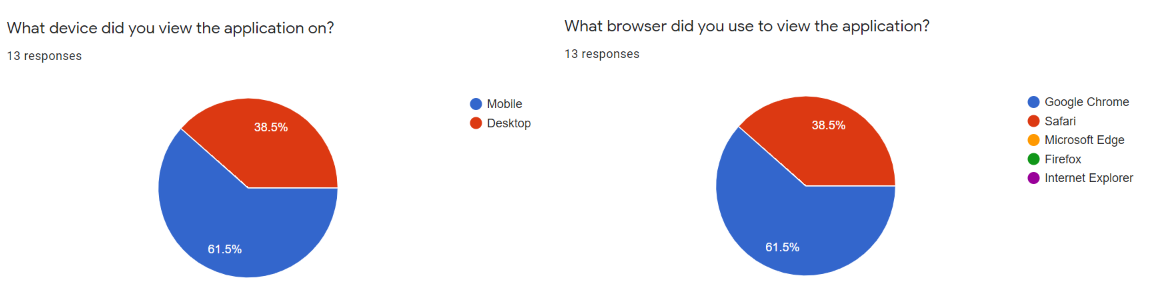
\includegraphics[width=0.95\textwidth]{figures/survey_results_device_browser.png}
    \caption{Device and browser used to access the application}
    \label{fig:SurveyResults}
\end{figure}

Respondents viewed the app on both mobile and desktop devices, and using two web browsers: Chrome and Safari. All had prior experience using the Dublin Bus service, and a majority had used other travel applications such as Google Maps and Moovit to plan journeys. The aggregate CSAT score \cite{CSAT} recorded from the survey was a 7 out of 10, outperforming the Dublin Bus iOS app (which has a score of only 2 out of 5 \cite{DublinBus-Reviews}).

Several respondents also provided more detailed feedback on the UI/UX of the application.
The layout of the map on the page was a prominent point of criticism, particularly the fact that a user must scroll past the map in order to view their search results.
One respondent also considered the search results themselves confusing, as the total journey time appears to be in the same format (HH:MM) as the expected time of arrival.

\subsection{Google Lighthouse}

\begin{figure}[!htb]
    \centering
    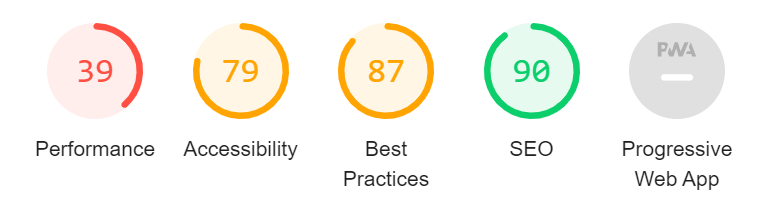
\includegraphics[width=0.7\textwidth]{figures/Google-Lighthouse_results_reduced.png}
    \caption{Google Lighthouse report results}
    \label{fig:GLResults}
\end{figure}

Google Lighthouse is an automated service available within the Chrome developer tools, which rates a web-page by its adherence to key features of progressive web apps \cite{Lighthouse}.
Performance gauges page-load efficiency; Accessibility quantifies the extent to which a page will be usable by all visitors; Best Practices checks for common mistakes; and SEO determines if the page is appropriately optimised to be crawled by search engines. These scores are achieved by a weighted average of key metric scores \cite{Lighthouse-Score}.

With some room for improvement, the application performs respectably in most categories, particularly SEO.
Some marks are lost for Accessibility due to insufficient colour contrast and a missing label on the Dark Mode toggle button.
However, the greatest room for improvement is in Performance, whose result of 39 is considered Poor.

Based on the Lighthouse evaluation results, and in the absence of results for back-end performance, one can conclude that the application’s greatest target for quality improvement is response time, which suffers from issues on the server-side and client-side.

\section{Data Analytics Evaluation}\label{DA-eval}

As mentioned in Chapter \ref{chapter4} random forest models were selected over linear regression and XGBoost models as they had promising results without the burden of excessive computational overhead.
Models were trained and tested on the first nine and final three months of the year respectively.

The development team agreed that an RMSE value of 300 seconds was acceptable for the random forest models.
It should be noted that outliers were removed only from the training set, causing error values to skew upwards when models were introduced to the testing set.
One would therefore expect the models' apparent error to be lower in practice than the error values in Figure \ref{fig:modelComparison} might indicate.
However, practical concerns made it impossible to test this hypothesis in the context of an undeployed app and testing this hypothesis is complicated by changes which may stem from the COVID19 pandemic and distinctly 2021 factors.

\begin{figure}[!htb]
    \centering
    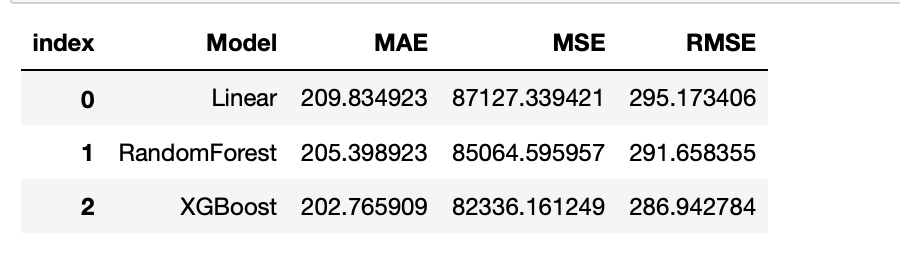
\includegraphics[width=0.7\textwidth]{figures/route_102_model_comparison.png}
    \caption{Error comparison for Linear Regression, Random Forest and XGBoost models trained on the data for Dublin Bus Route 102}
    \label{fig:modelComparison}
\end{figure}


\chapter{\label{chapter6}Major Contributions}


\chapter{\label{chapter7}Background Research}



\chapter{\label{chapter8} Critical Evaluation \& Future Work}




%%%% ADD YOUR BIBLIOGRAPHY HERE
\newpage
\begin{thebibliography}{99}
\bibitem{DAWSON:2000} Christian Dawson. \emph{The Essence of Computing Projects -- A Student's Guide}. 192 pages. ISBN: 013021972X. Pearson Education, 2000.

\bibitem{DublinBus-About} DublinBus \emph{Corporate Information}, accessed 22 August 2021, \href{https://www.dublinbus.ie/About-Us/}{https://www.dublinbus.ie/About-Us/}

\bibitem{TFI-BusTravel} Transport for Ireland \emph{About Bus Travel}, accessed 22 August 2021, \href{https://www.transportforireland.ie/getting-around/by-bus/about-bus-travel/}{https://www.transportforireland.ie/getting-around/by-bus/about-bus-travel/}

\bibitem{DublinBus-JourneyPlanner} DublinBus \emph{Journey Planner}, accessed 22 August 2021, \href{https://www.dublinbus.ie/Journey-Planner-iFrame/}{https://www.dublinbus.ie/Journey-Planner-iFrame/}

\bibitem{DublinBus-Schedule} DublinBus 46A Schedule \emph{46A Timetable}, accessed 22 August 2021, \href{https://www.dublinbus.ie/Your-Journey1/Timetables/All-Timetables/46a-2113/}{https://www.dublinbus.ie/Your-Journey1/Timetables/All-Timetables/46a-2113/}

\bibitem{Diab:2013} Diab, E.I., El-Geneidy, \emph{A.M. Variation in bus transit service: understanding the impacts of various improvement strategies on transit service reliability}. Public Transp 4, 209–231 (2013). \href{https://doi-org.ucd.idm.oclc.org/10.1007/s12469-013-0061-0}{https://doi-org.ucd.idm.oclc.org/10.1007/s12469-013-0061-0}

\bibitem{DublinBus-Reviews} App Store Reviews Various Users \emph{Dublin Bus - Ratings and Reviews}, accessed 22 August 2021, \href{https://apps.apple.com/ie/app/dublin-bus/id450455266#see-all/reviews}{ https://apps.apple.com/ie/app/dublin-bus/id450455266\#see-all/reviews}

\bibitem{DublinBus-Reviews-2} DublinBus Trustpilot Reviews Various Users \emph{Dublin Bus Reviews}, accessed 22 August 2021, \href{https://ie.trustpilot.com/review/dublinbus.ie}{https://ie.trustpilot.com/review/dublinbus.ie}

\bibitem{DublinBus-Reviews-3} DublinBus Google Play Reviews Various Users \emph{Dublin Bus - Apps on Google Play}, accessed 22 August 2021, \href{https://play.google.com/store/apps/details?id=com.dublinbus.wearei3&hl=en_IE&gl=US&showAllReviews=true}{https://play.google.com/store/apps/details?id=com.dublinbus.wearei3&hl=en_IE&gl=US&showAllReviews=true}

\bibitem{Zheng:2010} Zheng Li, David A. Hensher, John M. Rose (2010), \emph{Willingness to pay for travel time reliability in passenger transport: A review and some new empirical evidence}. Transportation Research Part E: Logistics and Transportation Review, Volume 46, Issue 3, Pages 384-403. ISSN 1366-5545 \href{https://doi.org/10.1016/j.tre.2009.12.005}{https://doi.org/10.1016/j.tre.2009.12.005}.

\bibitem{Yu:2018}Yu, B., Wang, H., Shan, W., & Yao, B. (2018). \emph{Prediction of Bus Travel Time Using Random Forests Based on Near Neighbors}. Computer-Aided Civil & Infrastructure Engineering, 33(4), 333–350. \href{https://doi-org.ucd.idm.oclc.org/10.1111/mice.12315}{https://doi-org.ucd.idm.oclc.org/10.1111/mice.12315}

\bibitem{Petersen_2019}Petersen, Niklas Christoffer and Rodrigues, Filipe and Pereira, Francisco Camara, (2019). \emph{Multi-output bus travel time prediction with convolutional LSTM neural network}. Expert Systems with Applications, Volume 120, Pages 426-435. ISSN 0957-4174, Elsevier BV. \href{http://dx.doi.org/10.1016/j.eswa.2018.11.028}{http://dx.doi.org/10.1016/j.eswa.2018.11.028}.

\bibitem{SVM}Bai, C., Peng, Z. R., Lu, Q. C., & Sun, J. (2015). \emph{Dynamic Bus Travel Time Prediction Models on Road with Multiple Bus Routes}. Computational intelligence and neuroscience, 2015, 432389.
\href{https://doi.org/10.1155/2015/432389}{https://doi.org/10.1155/2015/432389}.

\bibitem{RF}Moreira, J. P. C. L. M. (2008), \emph{Travel time prediction for the planning of mass transit companies: a machine learning approach}, Universidade do Porto, Porto, Portuguese Republic.
\href{https://core.ac.uk/download/pdf/143406304.pdf}{https://core.ac.uk/download/pdf/143406304.pdf}

\bibitem{TFI-App} Transport For Ireland \emph{TFI - Plan a Journey}, accessed 22 August 2021, \href{https://www.transportforireland.ie/plan-a-journey/}{https://www.transportforireland.ie/plan-a-journey/}

\bibitem{Moovit-App} Moovit \emph{Moovit Journey Planner}, accessed 22 August 2021, \href{https://moovitapp.com/ireland-502/poi/en-gb}{https://moovitapp.com/ireland-502/poi/en-gb}

\bibitem{GoogleMaps-App} Google Maps \emph{Google Maps}, accessed 22 August 2021, \href{https://www.google.com/maps}{https://www.google.com/maps}


\bibitem{TFI-Review} Transport For Ireland Reviews Various Users \emph{TFI - Ratings and Reviews}, accessed 22 August 2021, \href{https://apps.apple.com/ie/app/real-time-information/id590250800#see-all/reviews}{https://apps.apple.com/ie/app/real-time-information/id590250800\#see-all/reviews}

\bibitem{Moovit-Review} Moovit Reviews Various Users \emph{Moovit - Ratings and Reviews}, accessed 22 August 2021, \href{https://apps.apple.com/ie/app/moovit-all-transit-options/id498477945#see-all/reviews}{https://apps.apple.com/ie/app/moovit-all-transit-options/id498477945\#see-all/reviews}

\bibitem{GoogleMaps-Review} Google Maps Reviews Various Users \emph{Google Maps - Ratings and Reviews}, accessed 22 August 2021, \href{https://apps.apple.com/ie/app/google-maps/id585027354#see-all/reviews}{https://apps.apple.com/ie/app/google-maps/id585027354\#see-all/reviews}

\bibitem{Scrum-Guide} Ken Schwaber and Jeff Sutherland \emph{The Scrum Guide 2020}, accessed 22 August 2021, \href{https://scrumguides.org/scrum-guide.html}{https://scrumguides.org/scrum-guide.html}
\bibitem{SO-Survey} StackOverflow \emph{Developer Survey 2020 - Developer Roles}, accessed 22 August 2021, \href{https://insights.stackoverflow.com/survey/2020#developer-roles}{https://insights.stackoverflow.com/survey/2020\#developer-roles}
\bibitem{SO-SurveyFrontEnd} StackOverflow \emph{Developer Survey 2020 - Developer Roles}, accessed 22 August 2021, \href{https://insights.stackoverflow.com/survey/2020#technology-most-loved-dreaded-and-wanted-web-frameworks}{https://insights.stackoverflow.com/survey/2020\#technology-most-loved-dreaded-and-wanted-web-frameworks}

\bibitem{Gamification-Retention}Rapp, Amon and Hopfgartner, Frank and Hamari, Juho and Linehan, Conor and Cena, Federica \emph{Strengthening gamification studies: Current trends and future opportunities of gamification research}, International journal of human-computer studies, Volume 127, Pages 1-6. ISSN 1071-5819 \href{https://doi.org/10.1016/j.ijhcs.2018.11.007}{https://doi.org/10.1016/j.ijhcs.2018.11.007}

\bibitem{IPCC}P.R. Shukla, J. Skea, E. Calvo Buendia, V. Masson-Delmotte, H.-O. Pörtner, D. C. Roberts, P. Zhai, R. Slade, S. Connors, R. van Diemen, M. Ferrat, E. Haughey, S. Luz, S. Neogi, M. Pathak, J. Petzold, J. Portugal Pereira, P. Vyas, E. Huntley, K. Kissick, M. Belkacemi, J. Malley, (eds.), \emph{IPCC, 2019: Climate Change and Land: an IPCC special report on climate change, desertification, land degradation, sustainable land management, food security, and greenhouse gas fluxes in terrestrial ecosystems}. In press. \href{https://www.ipcc.ch/srccl/}{https://www.ipcc.ch/srccl/}

\bibitem{Epics} Max Rehkopf \emph{Stories, epics, and initiatives}, accessed 22 August 2021, \href{https://www.atlassian.com/agile/project-management/epics-stories-themes}{https://www.atlassian.com/agile/project-management/epics-stories-themes}

\bibitem{AtlassianUsage} Atlassian \emph{Customers}, accessed 22 August 2021, \href{https://www.atlassian.com/customers}{https://www.atlassian.com/customers}

\bibitem{COVID19}World Health Organisation \emph{Coronavirus 2019 Timeline}, accessed 22 August 2021,\href{https://www.who.int/emergencies/diseases/novel-coronavirus-2019/interactive-timeline}{https://www.who.int/emergencies/diseases/novel-coronavirus-2019/interactive-timeline}


\bibitem{BBC-Car}BBC \emph{How our daily travel harms the planet}, accessed 22 August 2021, \href{https://www.bbc.com/future/article/20200317-climate-change-cut-carbon-emissions-from-your-commute}{https://www.bbc.com/future/article/20200317-climate-change-cut-carbon-emissions-from-your-commute}


\bibitem{Tree}gov.uk \emph{10 Million Trees - Trees}, accessed 22 August 2021, \href{http://www.tenmilliontrees.org/trees/}{http://www.tenmilliontrees.org/trees/}

\bibitem{GOV}gov.uk \emph{How the discovery phase works}, accessed 22 August 2021, \href{https://www.gov.uk/service-manual/agile-delivery/how-the-discovery-phase-works}{https://www.gov.uk/service-manual/agile-delivery/how-the-discovery-phase-works}


\bibitem{CentralRepository}Atlassian \emph{Comparing Workflows}, accessed 22 August 2021, \href{https://www.atlassian.com/git/tutorials/comparing-workflows}{https://www.atlassian.com/git/tutorials/comparing-workflows} 

\bibitem{MET}MET Eireann \emph{Historical Data}, accessed 22 August 2021, \href{https://www.met.ie/climate/available-data/historical-data}{https://www.met.ie/climate/available-data/historical-data}

\bibitem{OpenWeatherMap}OpenWeatherMap \emph{History Bulk}, accessed 22 August 2021, \href{https://openweathermap.org/history-bulk}{https://openweathermap.org/history-bulk}

\bibitem{DataModel}Shung Gao,  \emph{Information System Analysis 6840 -  Data Modeling in System Analysis}, accessed 22 August 2021, \href{https://www.umsl.edu/~sauterv/analysis/Fall2010Papers/Gao/}{https://www.umsl.edu/~sauterv/analysis/Fall2010Papers/Gao/}

\bibitem{MD}Material Design,  \emph{Introduction}, accessed 23 August 2021, \href{https://material.io/design/introduction}{https://material.io/design/introduction}

\bibitem{Optaros} Stephen Walli, Dave Gynn, and Bruno Von Rotz, \emph{The Growth of Open Source Software in Organizations}, accessed 23 August 2021, \href{https://www.immagic.com/eLibrary/ARCHIVES/GENERAL/OPTAR_US/O051219W.pdf}{https://www.immagic.com/eLibrary/ARCHIVES/GENERAL/OPTAR_US/O051219W.pdf}


\bibitem{WhyDjango} Django, \emph{Django Overview}, accessed 23 August 2021, \href{https://www.djangoproject.com/start/overview/}{https://www.djangoproject.com/start/overview/}

\bibitem{WhyFlask} Flask, \emph{Flask Overview}, accessed 23 August 2021, \href{
https://flask.palletsprojects.com/en/2.0.x/}{https://flask.palletsprojects.com/en/2.0.x/}

\bibitem{XGB} Andrew Fogg, \emph{Anthony Goldbloom gives you the secret to winning Kaggle competitions}, accessed 23 August 2021, \href{https://www.import.io/post/how-to-win-a-kaggle-competition/}{https://www.import.io/post/how-to-win-a-kaggle-competition/}

\bibitem{CSAT} Qualtrics, \emph{What is CSAT}, accessed 23 August 2021, \href{https://www.qualtrics.com/uk/experience-management/customer/what-is-csat/}{https://www.qualtrics.com/uk/experience-management/customer/what-is-csat/}

\bibitem{Lighthouse} Google, \emph{What is Lighthouse}, accessed 23 August 2021, \href{https://developers.google.com/web/tools/lighthouse}{https://developers.google.com/web/tools/lighthouse}

\bibitem{Lighthouse-Score} Google, \emph{Lighthouse Performance Scoring}, accessed 23 August 2021, \href{https://web.dev/performance-scoring/}{https://web.dev/performance-scoring/}

\end{thebibliography}
\label{endpage}
\end{document}

\end{article}
